\documentclass[11pt]{article}

\usepackage[margin=1.0in]{geometry}
\usepackage{amsmath,amsthm,amssymb}
\usepackage{mathtools}
\usepackage{graphicx}
\usepackage{xcolor}
\usepackage{setspace}
\usepackage{multirow}
\usepackage{booktabs}
\usepackage{comment}
\usepackage{dsfont}
\usepackage{authblk}
\usepackage{lineno}
\usepackage{url}
\usepackage{appendix}
\usepackage{natbib}

\bibpunct{(}{)}{;}{a}{}{,}

\definecolor{NAU-Blue}{RGB}{0,51,102}        % NAU True Blue
\definecolor{NAU-Gold}{RGB}{241,179,0}       % NAU Gold

\definecolor{magenta-dark}{RGB}{140,0,140}   % High contrast
\definecolor{magenta-medium}{RGB}{200,0,200}
\definecolor{magenta-light}{RGB}{255,0,255}

\def\T{{\mathrm{\scriptscriptstyle T}}}
\def\spacingset#1{\renewcommand{\baselinestretch}{#1}\small\normalsize}

%\linenumbers
\spacingset{1.1}

\renewcommand*{\Authsep}{, }
\renewcommand*{\Authand}{\authorcr}   % \renewcommand*{\Authand}{, }
\renewcommand*{\Authands}{, }
\renewcommand*{\Affilfont}{\small\normalfont}

%\setlength{\authorsep}{2em}
\setlength{\affilsep}{1.6em}            % set the space between author and affiliation
\setlength{\bibsep}{3pt}


\title{\textbf{Time Series Analysis of Transit Ridership}\vspace{5pt}}

\author[1]{Rylan Harris}
\author[1]{Nick Larson}
\author[1]{Eli Vatsaas}

\affil[1]{Department of Mathematics and Statistics, Northern Arizona University, Flagstaff, AZ 86011, USA}

\date{\today}

%------------------------------------------------------------------------------%
\begin{document}
%------------------------------------------------------------------------------%

\maketitle

\begin{abstract}
This study applies time series analysis techniques to investigate patterns in public transit ridership in the United States, with particular attention to the impact of COVID-19. Using monthly Unlinked Passenger Trips (UPT) data from the National Transit Database spanning January 2002 to February 2025, we develop multiple time series models using both manual and automated approaches at national and jurisdictional levels. Our methodology includes fitting SARIMA models to pre-COVID data to estimate counterfactual ridership levels and developing intervention models to capture the structural break caused by the pandemic. Results indicate that while transit ridership follows consistent seasonal patterns, COVID-19 caused unprecedented disruption to ridership levels. Although recovery has occurred, current ridership remains significantly below pre-pandemic forecasted levels, with the recovery rate showing signs of deceleration. The jurisdictional analysis reveals geographical variations in both pre-pandemic patterns and post-pandemic recovery trajectories. This analysis provides valuable insights for transit agencies and policymakers in understanding ridership patterns and the long-term implications of major disruptions on public transportation systems.
\end{abstract}

\vspace{8pt}
\noindent
\textbf{Keywords}: Time series analysis; SARIMA models; Public transportation; COVID-19 impact; Ridership forecasting; Intervention analysis.

%------------------------------------------------------------------------------%
\section{Introduction}
%------------------------------------------------------------------------------%

Public transit systems represent critical infrastructure in urban environments, supporting economic activity, reducing traffic congestion, and providing essential mobility for millions of Americans. Understanding patterns and trends in transit ridership is crucial for effective planning, resource allocation, and policy development. The COVID-19 pandemic that emerged in early 2020 created an unprecedented disruption to transit systems nationwide, with dramatic declines in ridership as lockdown measures were implemented and remote work became widespread.

This study explores patterns in transit ridership across the United States using time series analysis techniques, with particular attention to the impact of COVID-19. Specifically, we examine monthly Unlinked Passenger Trips (UPT) data collected by the Federal Transit Administration to develop models that can characterize ridership patterns, forecast future trends, and quantify the pandemic's effects. This analysis provides valuable insights into both typical transit usage patterns and the magnitude and persistence of major disruptions.

Transit ridership typically follows predictable seasonal patterns, with variations based on weather, holidays, academic calendars, and other cyclical factors. These patterns create natural opportunities for time series modeling approaches, while the scale of disruption caused by COVID-19 presents a unique case study for understanding how major external shocks impact established transportation patterns and how systems recover from such events.

Our analysis employs multiple complementary approaches:

\begin{enumerate}
  \item \textbf{Pre-COVID SARIMA Model:} We develop a seasonal autoregressive integrated moving average (SARIMA) model using pre-pandemic data to establish a counterfactual forecast of what ridership would have been without COVID-19.
  
  \item \textbf{Intervention Model:} We develop an intervention model that incorporates the entire range of dates available to create a model that can account for the influence of COVID-19 to more accurately forecast future values.
  
  \item \textbf{Jurisdiction-Specific Analysis:} Using the national models as a basis, we apply these methods programmatically across each individual jurisdiction and look at the patterns in the models made.
  
\end{enumerate}

The findings from this study have important implications for transit agencies, urban planners, and policymakers as they work to understand ridership patterns, rebuild from disruptions, adapt service models, and prepare for future challenges. By employing multiple modeling approaches at different geographical scales, we provide a comprehensive analysis of public transportation usage patterns and resilience.

%------------------------------------------------------------------------------%
\section{The Data}
%------------------------------------------------------------------------------%

This study utilizes monthly Unlinked Passenger Trips (UPT) data from the National Transit Database (NTD) maintained by the Federal Transit Administration. The dataset covers the period from January 2002 through February 2025, providing a comprehensive longitudinal view of transit ridership patterns across the United States. UPT represents the number of passengers who board public transportation vehicles, regardless of whether a passenger is transferring from another vehicle. It serves as a standard metric for measuring transit system usage.

The raw data was obtained from the Monthly Module Raw Data Release available on the Federal Transit Administration's website (https://www.transit.dot.gov/ntd/data-product/monthly-module-raw-data-release). In its original format, the dataset presented each jurisdiction-transit mode combination as a separate row, with monthly UPT figures arranged across columns. This structure required significant preprocessing before analysis could begin.

\subsection{Data Cleaning and Preparation}

The data cleaning process involved several key steps:

\begin{enumerate}
  \item \textbf{Restructuring to tidy format:} We transformed the data so that each row represents a single observation (one month's UPT for a specific jurisdiction-mode combination). This required parsing the column names to extract month and year information and converting these into proper date objects.
  
  \item \textbf{Aggregation by jurisdiction:} We aggregated the data by summing UPT values across different transit modes within each jurisdiction to obtain jurisdiction-level totals.
  
  \item \textbf{Removing incomplete data:} We filtered the data to only include jurisdictions that had complete data. This maintained a reasonable number and ensured consistency across our analysis.
  
  \item \textbf{National aggregation:} For the nationwide analysis, we further aggregated these filtered jurisdiction-level totals to produce monthly national UPT figures.
\end{enumerate}

\begin{figure}[!ht]
\centering

\includegraphics[width=0.525\linewidth]{Total_UPT_trend.png}
\caption{Monthly national UPT from January 2002 to February 2025, showing seasonal patterns and COVID-19 disruption}
\label{f:data}
\end{figure}

Visual inspection of the national UPT time series (Figure~\ref{f:data}) reveals strong seasonal patterns, with consistent yearly cycles. The data shows relatively stable ridership levels for many years prior to 2020, followed by a dramatic decline coinciding with the onset of the COVID-19 pandemic in early 2020. This abrupt change represents the most significant disruption in the 23-year period covered by our dataset.

\subsection{Data Quality Assessment}

Data quality checks revealed some missing values and outliers, particularly for smaller transit agencies during certain months. These issues were addressed by excluding jurisdictions with missing values. The original set had a total of 828 jurisdictions, filtered into 197 of them with complete data. This spanned four modes of transport: bus, rail, ferry, and other. As a result, the national aggregated data used for our primary models showed no significant gaps or anomalies outside of the expected pandemic-related disruption.

\begin{figure}[!ht]
\centering
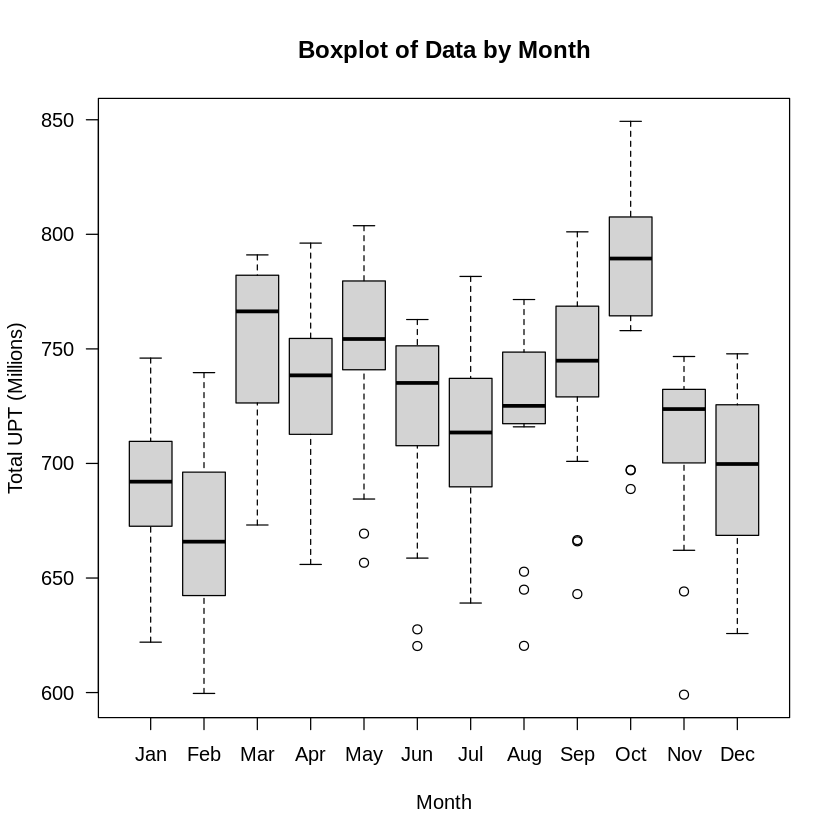
\includegraphics[width=0.525\linewidth]{seasonal_trend.png}
\caption{Seasonal patterns in national transit ridership (UPT by month)}
\label{f:seasonal}
\end{figure}

The extensive time period covered by this dataset allows us to establish robust baseline models of pre-pandemic ridership patterns while also capturing the full trajectory of the pandemic's impact and the subsequent recovery period. This temporal scope is essential for addressing our research questions regarding both typical ridership patterns and the effects of major disruptions.

%------------------------------------------------------------------------------%
\section{Methods}
%------------------------------------------------------------------------------%

Our analysis employed multiple time series modeling approaches to understand transit ridership patterns and the impact of COVID-19. This section details the methods used for the pre-COVID forecast model development, the intervention model, and how we applied those procedures across each individual jurisdiction.

\subsection{Data Preparation}

After restructuring the raw data into a tidy format as described in Section 2, we conducted several diagnostic procedures to ensure the data was suitable for time series analysis. First, we examined the national pre-COVID UPT time series for trends, seasonality, and potential outliers through visual inspection of time plots. This initial examination revealed strong seasonal patterns with annual periodicity.

\begin{figure}[!ht]
\centering
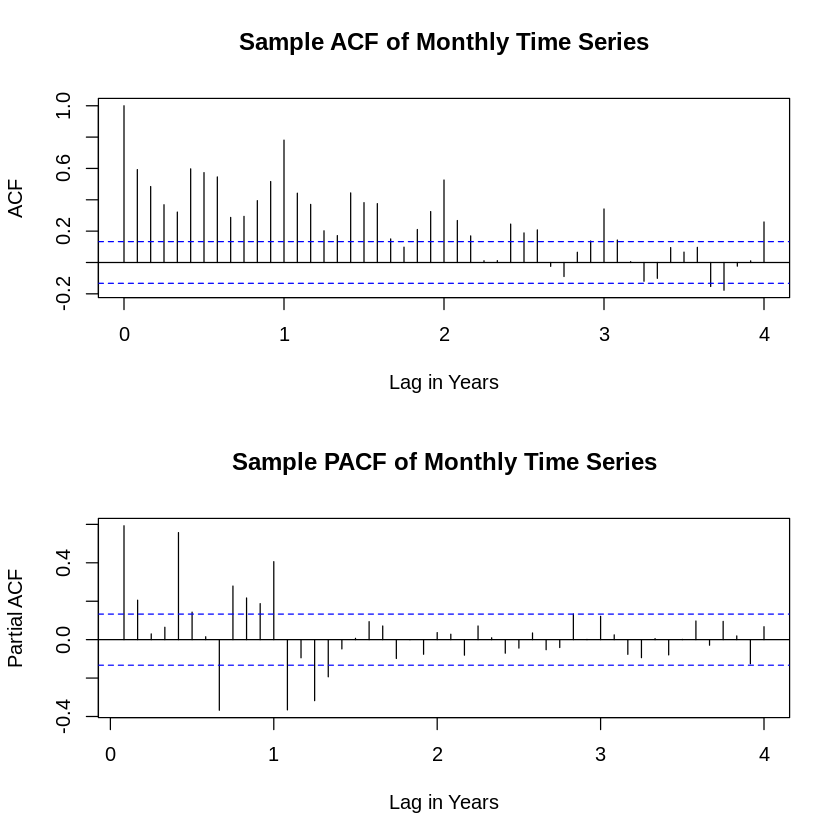
\includegraphics[width=0.525\linewidth]{pre_acf_pacf.png}
\caption{ACF and PACF of the original UPT time series}
\label{f:acf_pacf_orig}
\end{figure}

To prepare the data for modeling, we performed the following steps:

\begin{enumerate}
  \item Applied a natural logarithm transformation to stabilize variance across the time series, as the magnitude of seasonal fluctuations showed proportionality to the level of the series.
  
  \item Conducted an Augmented Dickey-Fuller (ADF) test to formally assess stationarity of the transformed series. The test results were as follows:
  
  Dickey-Fuller = -1.8252, Lag order = 5, p-value = 0.6493 (note: alternative hypothesis: stationary)
  
  The test statistic confirmed our visual assessment that the series was non-stationary.
  
  \item Performed seasonal differencing (lag-12) to address the strong annual seasonality in the data.
  
  \item Conducted an additional Augmented Dickey-Fuller (ADF) test to formally assess stationarity of the now differenced series. The test results were as follows:
  
  Dickey-Fuller = -15.679, Lag order = 5, p-value = 0.01
  
  The test statistic confirmed our visual assessment that the series was non-stationary.
  
  \item Applied first-order differencing to address the remaining trend component after seasonal differencing.
\end{enumerate}

\begin{figure}[!ht]
\centering

\includegraphics[width=0.525\linewidth]{diff_series.png}
\caption{Log-transformed series after first-order and seasonal differencing}
\label{f:diff_series}
\end{figure}

These transformations resulted in a stationary series appropriate for SARIMA modeling, as confirmed by both visual inspection and statistical testing.

\subsection{Pre-COVID Model Development}

To estimate the impact of COVID-19 on transit ridership, we developed a forecasting model using only pre-pandemic data (January 2002 through January 2020). This approach allowed us to project what ridership would have been in the absence of the pandemic, creating a counterfactual for comparison with actual ridership figures.

\begin{figure}[!ht]
\centering
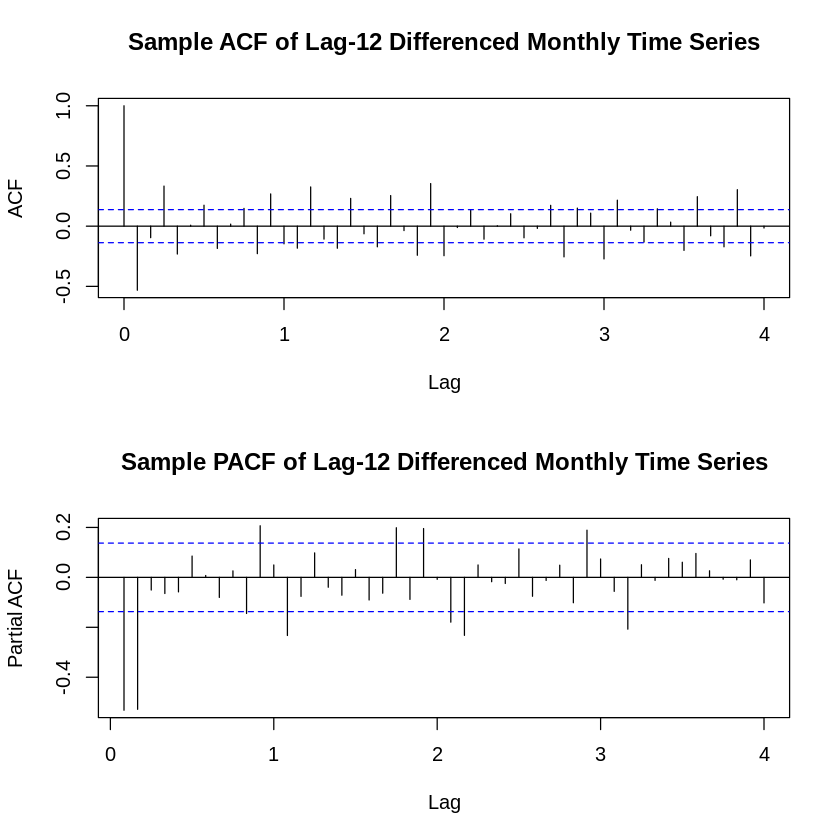
\includegraphics[width=0.525\linewidth]{diff_acf_pacf.png}
\caption{ACF and PACF of the differenced log-transformed series}
\label{f:acf_pacf_diff}
\end{figure}

Model selection proceeded through the following steps:

\begin{enumerate}
  \item Examined the Autocorrelation Function (ACF) and Partial Autocorrelation Function (PACF) of the differenced log-transformed series to identify potential SARIMA model specifications (Figure~\ref{f:acf_pacf_diff}).
  
  \item Based on the patterns observed in the ACF and PACF, we identified several candidate SARIMA models.
  
  \item Estimated multiple SARIMA models with varying orders and compared their performance using the Akaike Information Criterion with correction for small sample size (AICc), as shown in Table~\ref{t:model_comparison}.
  
  \item Selected the SARIMA$(2,1,0)\times(1,1,1)_{12}$ model as our final specification based on having the lowest AICc value among the candidate models. This model can be written as:
\end{enumerate}

\begin{equation}
y_t = \phi_1 y_{t-1} + \phi_2 y_{t-2} + \Phi_1 y_{t-12} - \phi_1\Phi_1 y_{t-13} - \phi_2\Phi_1 y_{t-14} + y_{t-1} - y_{t-13} + \varepsilon_t + \Theta_1 \varepsilon_{t-12}
\end{equation}

where $y_t$ represents the natural logarithm of UPT at time $t$, $\phi_1$ and $\phi_2$ are non-seasonal autoregressive parameters, $\Phi_1$ is the seasonal autoregressive parameter, $\Theta_1$ is the seasonal moving average parameter, and $\varepsilon_t$ is white noise.

\begin{table}[!ht]
\caption{Comparison of candidate SARIMA models}
\label{t:model_comparison}
\begin{center}
\begin{tabular}{lccc}
\hline
Model & AICc & BIC\\
\hline
SARIMA(1,1,1)×(1,1,1)$_{12}$ & -903.5658 & -887.1639 \\
SARIMA(0,1,1)×(0,1,1)$_{12}$ & -883.9929 & -874.1517 \\
SARIMA(1,1,0)×(1,1,0)$_{12}$ & -805.1018 & -795.2607 \\
SARIMA(0,1,1)×(1,1,0)$_{12}$ & -847.2331 & -837.3919 \\
SARIMA(1,1,0)×(0,1,1)$_{12}$ & -851.4125 & -841.5713 \\
SARIMA(2,1,0)×(1,1,1)$_{12}$ & -924.1164 & -907.7145 \\
SARIMA(1,1,0)×(1,1,1)$_{12}$ & -861.8188 & -848.6972 \\
SARIMA(2,1,1)×(1,1,1)$_{12}$ & -922.1399 & -902.4576 \\
\hline
\end{tabular}
\end{center}
\end{table}

The selected model was then used to generate forecasts for the period from February 2020 through February 2025, representing our estimate of what transit ridership would have been without the COVID-19 disruption. To facilitate interpretation, these forecasts were transformed back to the original scale (UPT counts) and accompanied by 95\% prediction intervals to account for forecast uncertainty.

\subsection{Impact Assessment}

To quantify the impact of COVID-19 on transit ridership, we calculated the difference between the forecasted values from our pre-COVID model and the actual observed ridership for each month from February 2020 onward. These differences represent our estimate of ridership loss attributable to the pandemic. Both absolute differences (in terms of UPT counts) and percentage differences relative to the forecast were computed to provide a comprehensive view of the impact.

Additionally, we examined the pattern of these differences over time to assess the trajectory of recovery. This analysis involved investigating whether the gap between forecasted and actual ridership was narrowing and at what rate, providing insights into the persistent effects of the pandemic on transit usage patterns.

\subsection{Intervention Model Development}

To properly account for the COVID-19 pandemic's impact on transit ridership patterns, we developed an intervention model that incorporated data through the pandemic. Unlike the pre-COVID model that used only data through January 2020, this approach explicitly models the pandemic's effect through an intervention variable.

This intervention variable $X_t$ was defined as:

\begin{equation}
X_t = 
\begin{cases}
0, & \text{for } t < \text{February 2020} \\
1, & \text{for } t \geq \text{February 2020}
\end{cases}
\end{equation}

This specification treats the pandemic as a permanent level shift, reflecting the persistence of its effects on transit ridership patterns.

\subsubsection{Full Data and Stationarity Analysis}

Applying the same differencing as the pre-COVID model, along with the same log transformation was all that was needed for stationary data. Figure \ref{fig:diff_full_series} displays the resulting differenced series.

\begin{figure}[!ht]
\centering

\includegraphics[width=0.8\textwidth]{diff_series_full.png}
\caption{Log-transformed series after first-order and seasonal differencing}
\label{fig:diff_full_series}
\end{figure}

The differenced series fluctuates around zero with relatively stable variance until early 2020, when the COVID-19 pandemic causes a dramatic spike. This confirms a need for an intervention approach rather than trying to model this structural break through standard SARIMA analysis alone.

\subsubsection{Model Selection Process}

To identify the optimal intervention model, we proceeded through the following steps:

\begin{enumerate}
\item Examined the Autocorrelation Function (ACF) and Partial Autocorrelation Function (PACF) of the differenced log-transformed series to identify potential SARIMA model specifications with intervention (Figure \ref{fig:acf_pacf_diff}).

\item Based on the patterns observed in the ACF and PACF, we identified several candidate SARIMA models with the COVID-19 intervention variable.

\item Estimated multiple SARIMA models with varying orders and compared their performance using the Akaike Information Criterion with correction for small sample size (AICc), as shown in Table \ref{tab:intervention-models}.

\item Selected the SARIMA(1, 1, 3) × (0, 1, 1)$_{12}$ model with COVID intervention as our final specification based on having the lowest AICc value among the candidate models.
\end{enumerate}

\begin{figure}[!ht]
\centering
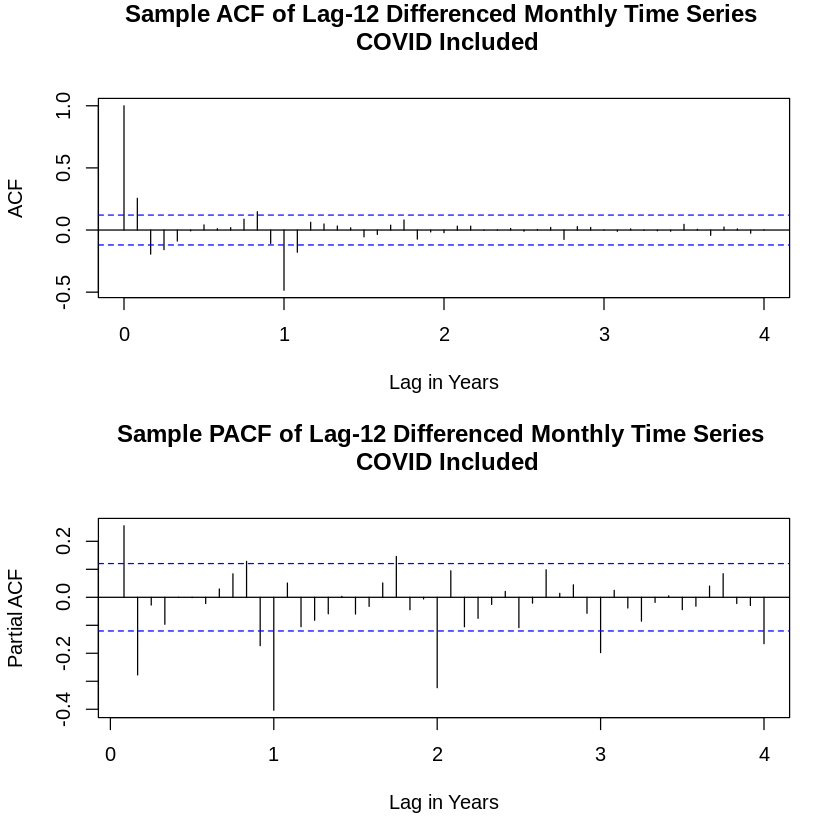
\includegraphics[width=0.8\textwidth]{diff_acf_pacf_full.png}
\caption{ACF and PACF of the differenced log-transformed series}
\label{fig:acf_pacf_diff}
\end{figure}

\begin{table}[!ht]
\centering
\caption{Comparison of candidate SARIMA models with COVID intervention}
\label{tab:intervention-models}
\begin{tabular}{lrr}
\hline
Model & AICc & BIC \\
\hline
SARIMA(1,1,1)×(1,1,1)$_{12}$ & -546.6943 & -525.8355 \\
SARIMA(0,1,1)×(0,1,1)$_{12}$ & -549.9856 & -536.0134 \\
SARIMA(1,1,0)×(1,1,0)$_{12}$ & -436.0365 & -422.0643 \\
SARIMA(0,1,1)×(1,1,0)$_{12}$ & -481.2186 & -467.2463 \\
SARIMA(1,1,0)×(0,1,1)$_{12}$ & -518.3117 & -504.3395 \\
SARIMA(1,1,2)×(0,1,1)$_{12}$ & -547.1353 & -526.2764 \\
SARIMA(1,1,3)×(0,1,1)$_{12}$ & -579.8213 & -555.5447 \\
\hline
\end{tabular}
\end{table}

We selected the SARIMA(1,1,3)$\times$(0,1,1)$_{12}$ model as our final specification based on it having the lowest AICc value (-579.8213) among all candidate models and passing the Ljung-Box test for residual autocorrelation.

The selected intervention model can be written as:
\begin{equation}
(1 - \phi_1 B)(1 - B)(1 - B^{12})y_t = (1 + \theta_1 B + \theta_2 B^2 + \theta_3 B^3)(1 + \Theta_1 B^{12})\varepsilon_t + \beta X_t
\end{equation}

which expands to:
\begin{equation}
\begin{split}
y_t &= y_{t-1} + \phi_1(y_{t-1} - y_{t-2}) + y_{t-12} - y_{t-13} - \phi_1(y_{t-13} - y_{t-14}) \\
&+ \varepsilon_t + \theta_1\varepsilon_{t-1} + \theta_2\varepsilon_{t-2} + \theta_3\varepsilon_{t-3} + \Theta_1\varepsilon_{t-12} + \theta_1\Theta_1\varepsilon_{t-13} \\
&+ \theta_2\Theta_1\varepsilon_{t-14} + \theta_3\Theta_1\varepsilon_{t-15} + \beta X_t
\end{split}
\end{equation}
where $y_t$ represents the natural logarithm of UPT at time $t$, $\phi_1$ is the non-seasonal autoregressive parameter, $\theta_1$, $\theta_2$, and $\theta_3$ are the non-seasonal moving average parameters, $\Theta_1$ is the seasonal moving average parameter, $\beta$ is the coefficient for the COVID intervention variable, and $\varepsilon_t$ is white noise.

Diagnostic checks confirm the adequacy of the model. The model passed the Ljung-Box test with a $p-value = 0.89$ ($df = 19$), confirming the model successfully captures the autocorrelation in the data. Visual inspection of the model residuals show no apparent patterns or heteroscedasticity. While a notable spike in residuals occurs at the pandemic onset, the intervention variable successfully captures this structural break, with well-behaved residuals before and after this event. This confirms appropriate model specification despite the structural break caused by the pandemic.

\subsection{Jurisdiction-Specific Analysis}

Since our initial consideration of this data, we knew that transit systems across the country would show vastly different ridership patterns. New York's subway system operates nothing like the bus network in Flagstaff, Arizona. With this in mind, we wanted to fit individual models to each jurisdiction to supplement our national investigation.

\subsubsection{Model Selection Strategy}

Early attempts at manual model selection for the 197 complete jurisdictions proved challenging. We weren't confident \textit{auto.arima} would give us accurate models. After trying various semi-automated approaches, we developed a comprehensive search algorithm that systematically explores SARIMA configurations. The automation decision comes from practical necessity - as manually selecting two separate model types for 197 jurisdictions was not feasible.


To avoid overfitting, we forced the following parameter limits:
\begin{itemize}
  \item Non-seasonal AR terms ($p$): limited to 0-5
  \item   Non-seasonal differencing term ($d$): set to 1
  \item Non-seasonal MA terms ($q$): limited to 0-5  
  \item Seasonal AR parameters ($P$): limited to 0-2
  \item   Seasonal differencing term ($D$): set to 1
  \item Seasonal MA terms ($Q$): limited to 0-2
  \item Ensured $p + q + P + Q \leq 5$
\end{itemize}

These restrictions served dual purposes: preventing models from fitting noise rather than genuine autocorrelation patterns, and maintaining reasonable computational requirements. By limiting model complexity, we improved forecast reliability while also ensuring the analysis could be completed within practical timeframes.

\subsubsection{Pre-COVID Model Development}

For each jurisdiction's pre-pandemic period (January 2002 through January 2020), we fit:

\begin{equation}
\text{SARIMA}(p,1,q) \times (P,1,Q)_{12}
\end{equation}

The CSS-ML  method  was used as our estimation approach, , using conditional sum of squares to provide starting estimations for model parameters before using maximum likelihood estimations to determine the final parameters. This hybrid technique, though slightly less elegant when compared to \textit{auto.arima}, proved robust across our diverse jurisdictions. 

Model selection relied on corrected AIC scores:

\begin{equation}
\text{AICc} = \text{AIC} + \frac{2k(k+1)}{n-k-1}
\end{equation}

where $k$ counts parameters and $n$ represents sample size. The AICc helps prevent the selection of overly complex models that may appear to fit well but have poor predictive performance. We then attempted to select the model with the lowest AICc while passing a Ljung-Box test. If one couldnt be passsed, we took the lowest AICc. 

\subsubsection{Intervention Model Framework}

To account for COVID-19's impact on transit ridership patterns, we incorporated an external intervention variable into our SARIMA models. This approach allowed us to quantify the pandemic's effect while maintaining the underlying time series structure:

\begin{equation}
\text{SARIMA}(p,1,q) \times (P,1,Q)_{12} \text{ with COVID intervention}
\end{equation}

The intervention variable was defined as:
\begin{equation}
X_t = \begin{cases}
0, & \text{for } t < \text{February 2020} \\
1, & \text{for } t \geq \text{February 2020}
\end{cases}
\end{equation}

This binary specification captures the abrupt shift in ridership patterns coinciding with pandemic-related restrictions in March 2020. The coefficient on this intervention variable directly measures the magnitude of COVID-19's impact on ridership levels for each jurisdiction, while the SARIMA components continue to model the temporal dynamics and seasonality of the transformed series. We then attempted to select the model with the lowest AICc while passing a Ljung-Box test. If one couldnt be passsed, we took the lowest AICc.

%------------------------------------------------------------------------------%
\section{Results}
%------------------------------------------------------------------------------%

Our time series analysis reveals the profound and persistent impact of the COVID-19 pandemic on public transit ridership across the United States. This section presents the key findings from our pre-COVID forecasting model and quantifies the deviation between projected and actual ridership levels.

\subsection{Pre-COVID Model Performance}

The SARIMA$(2,1,0)\times(1,1,1)_{12}$ model fitted to pre-pandemic data (January 2002 through January 2020) demonstrated strong performance in capturing the historical patterns of transit ridership. Table~\ref{t:model_params} presents the estimated parameters for this model, all of which were statistically significant at the 0.05 level.

\begin{table}[!ht]
\caption{Parameter estimates for the pre-COVID SARIMA model}
\label{t:model_params}
\begin{center}
\begin{tabular}{lcccc}
\hline
Parameter & Estimate & Std. Error & z value & p-value \\
\hline
$\phi_1$   & -0.831033 &  0.061180 & -13.5833 & $< 2.2e-16$ \\
$\phi_2$   & -0.530607 &  0.061499 &  -8.6279 & $< 2.2e-16$ \\
$\Phi_1$   &  0.261454 &  0.091259 &   2.8650 &  0.004171   \\
$\Theta_1$ & -0.918776 &  0.089919 & -10.2178 & $< 2.2e-16$ \\
\hline
\end{tabular}
\end{center}
\end{table}

Diagnostic checks of the model show that it is somewhat inadequate. The Ljung-Box test supports the alternative hypothesis of autocorrelation in the residuals (Q* = 38.457, df = 20, p-value = 0.007783), indicating that the model fails to captured the entirety of autocorrelation in the data. This is further shown in the ACF and PACF having several outstanding points. Visual inspection of the residuals showed no apparent patterns or heteroscedasticity and the residuals appear to be approximately normally distributed. This model was still selected as the most appropriate model despite its flaws for a few reasons. Given the nature of real-world data, trade-offs need to be made in order to avoid overfitting and maintaining interpretability. The significant parameters and the satisfactory features of the residuals support the overall adequacy for our forecasting purpose.

\subsection{Pandemic Impact Assessment}

Figure~\ref{f:forecast} illustrates the forecasted ridership levels from our pre-COVID model alongside the actual observed values from February 2020 onward. The dramatic divergence at the beginning of the pandemic clearly demonstrates the immediate and severe impact on transit usage.

\begin{figure}[!ht]
\centering
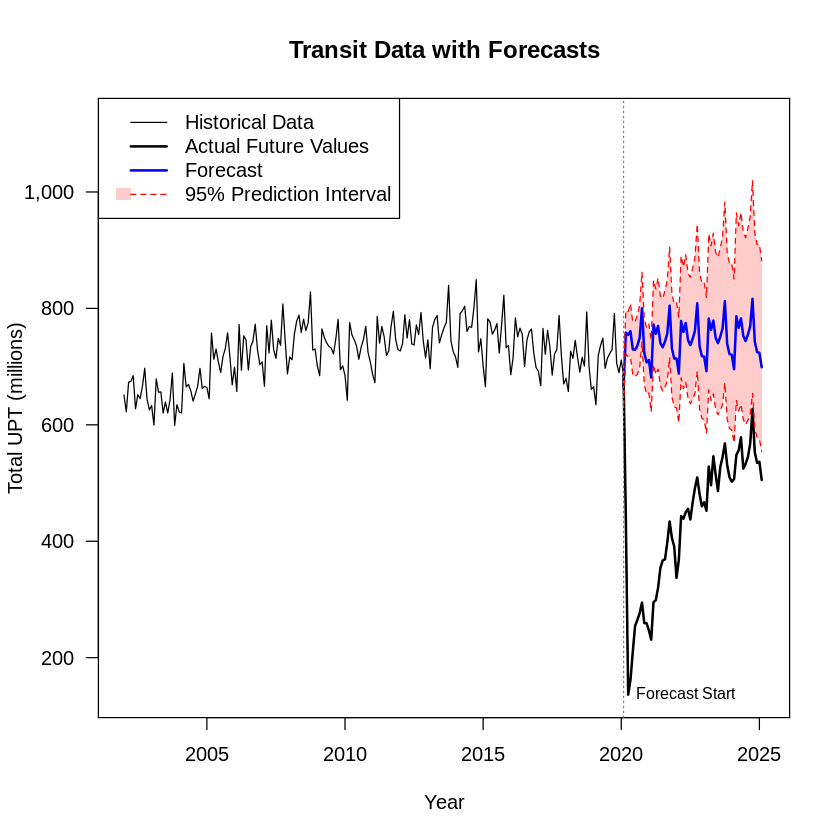
\includegraphics[width=0.485\linewidth]{pre_forecast.png}
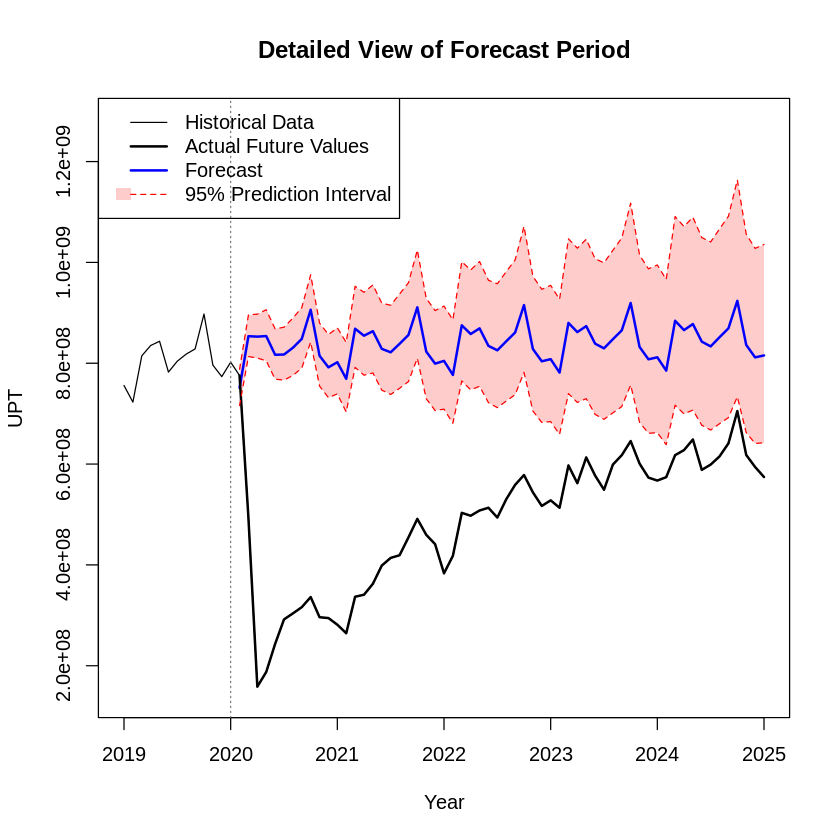
\includegraphics[width=0.485\linewidth]{pre_forecast_close.png}
\caption{National transit ridership: Pre-COVID forecast vs. actual values}
\label{f:forecast}
\end{figure}

The estimated ridership loss, computed as the difference between forecasted and actual UPT, is visualized in Figure~\ref{f:loss}. In the initial months of the pandemic (February-April 2020), ridership fell to approximately 20\% of expected levels, representing an unprecedented collapse in transit usage. 

\begin{figure}[!ht]
\centering
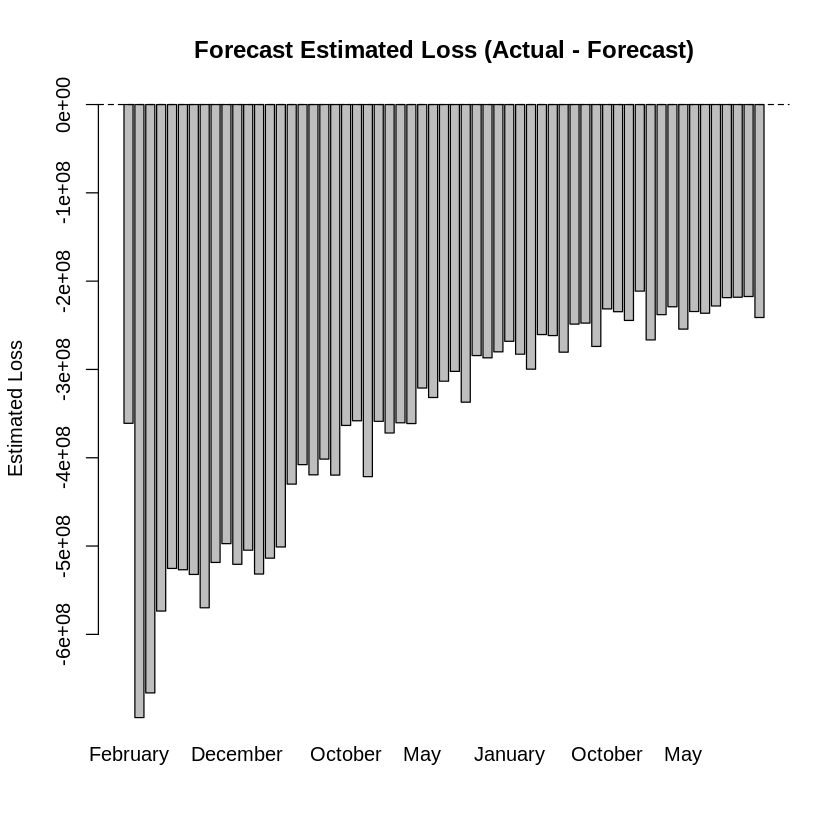
\includegraphics[width=0.525\linewidth]{estimated_loss.png}
\caption{Estimated monthly ridership loss due to COVID-19}
\label{f:loss}
\end{figure}

\subsection{Recovery Trajectory}

Analysis of the gap between forecasted and actual ridership over time reveals a gradual but incomplete recovery. By February 2025, the most recent month in our dataset, actual ridership remained notably lower, approximately 20\%, below the forecast level. This represents a significant improvement from the worst of the pandemic but indicates that transit ridership has not yet returned to its pre-pandemic trajectory.

The recovery pattern shows three distinct phases:
\begin{enumerate}
  \item Initial severe impact (February-May 2020): Characterized by the steepest decline in ridership, corresponding to widespread lockdowns and service reductions.
  \item Gradual recovery (June 2020-December 2021): Marked by steady improvement as restrictions eased and transit agencies restored service.
  \item Plateauing recovery (January 2022-February 2025): Showing slower improvement rates and signs of stabilization at a new, lower equilibrium level.
\end{enumerate}

As can be seen in Figure~\ref{f:forecast}, the actual ridership remains consistently below even the lower bound of the 95\% prediction interval of our forecast model, indicating that the pandemic's impact may represents a permanent shift in transit usage rates rather than a temporary anomaly within the expected range of variation.

The slowing rate of recovery in the most recent months suggests that some portion of the ridership loss may be permanent or at least persistent over a multi-year timeframe. This finding has significant implications for transit agencies' long-term planning and financial sustainability.

\subsection{Model Performance and Parameter Estimates}

Our intervention model, SARIMA(1,1,3)$\times$(0,1,1)$_{12}$ with a binary intervention variable for COVID-19, demonstrated strong performance in capturing both the pre-pandemic patterns and the structural break caused by COVID-19. Table~\ref{tab:intervention_params} presents the estimated parameters for this model, all of which were statistically significant.

\begin{table}[!ht]
\centering
\caption{Parameter estimates for the intervention SARIMA model}
\label{tab:intervention_params}
\begin{tabular}{lrrrr}
\hline
Parameter & Estimate & Std. Error & $z$ value & $p$-value \\
\hline
$\phi_1$ (ar1) & 0.9301 & 0.0283 & 32.8656 & $<$ 0.0001 \\
$\theta_1$ (ma1) & -1.7973 & 0.0718 & -25.0320 & $<$ 0.0001 \\
$\theta_2$ (ma2) & 0.7592 & 0.1337 & 5.6784 & $<$ 0.0001 \\
$\theta_3$ (ma3) & 0.1015 & 0.0722 & 1.4059 & 0.1598 \\
$\Theta_1$ (sma1) & -0.9119 & 0.0490 & -18.6102 & $<$ 0.0001 \\
$\beta$ (COVID) & -1.3321 & 0.0235 & -56.6851 & $<$ 0.0001 \\
\hline
\end{tabular}
\end{table}

The intervention coefficient ($\beta = -1.3321$) quantifies the magnitude of the pandemic's immediate impact on transit ridership. This coefficient indicates that, after accounting for existing temporal patterns, COVID-19 caused an immediate reduction of approximately 74\% ($1 - e^{-1.3321} \approx 0.736$) in transit ridership. The high statistical significance of this parameter ($p < 0.0001$) confirms the profound effect of the pandemic on transit usage patterns.


\subsection{Forecast Performance}

Figure~\ref{f:intervention_forecast} illustrates the performance of our intervention model in forecasting transit ridership for the twelve-month holdout period from March 2024 through February 2025. The model successfully captures the overall level and seasonal pattern of ridership during this period, although some deviations in exist specific months.

\begin{figure}[!ht]
\centering
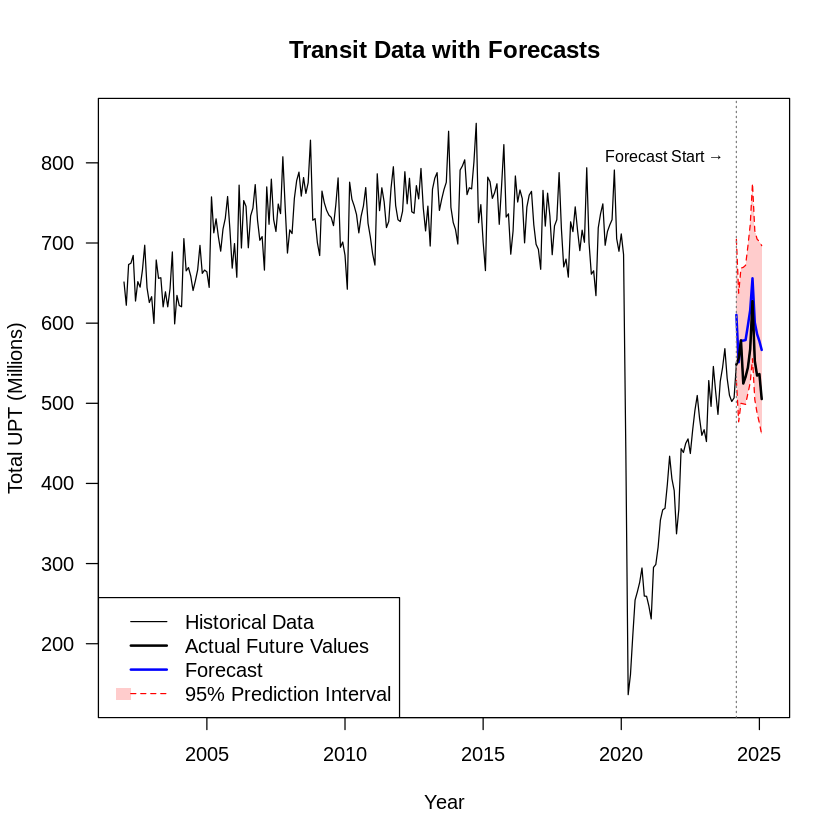
\includegraphics[width=0.485\linewidth]{forecast_post.png}
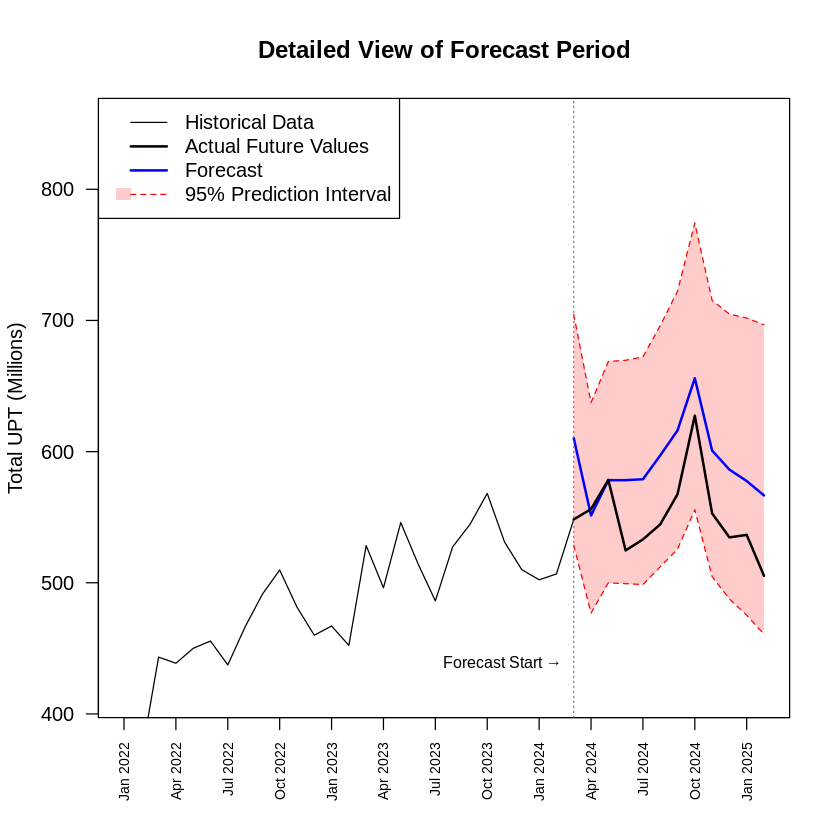
\includegraphics[width=0.485\linewidth]{forecast_post_close.png}
\caption{National transit ridership: COVID intervention forecast vs. actual values}
\label{f:intervention_forecast}
\end{figure}

Table~\ref{tab:forecast_accuracy} presents the forecast accuracy metrics for the intervention model during the holdout period. The model demonstrates good predictive performance with a Mean Absolute Percentage Error (MAPE) of $7.66\%$.

\begin{table}[!ht]
\centering
\caption{Forecast accuracy metrics for the intervention model (Mar 2024--Feb 2025)}
\label{tab:forecast_accuracy}
\begin{tabular}{lr}
\hline
Metric & Value \\
\hline
MAPE (\%) & 7.66 \\
RMSE (millions) & 45.81 \\
MAE (millions) & 41.51 \\
\hline
\end{tabular}
\end{table}

\subsection{Intervention Interpretation and Implications}

The intervention model results demonstrate that while transit ridership has partially recovered from the initial shock of the COVID-19 pandemic, it remains significantly below pre-pandemic levels. As seen visually, and confirmed by the coefficient of the COVID intervention, immediate impact of the pandemic in early 2020 was severe, with ridership dropping to approximately $25\%$ of pre-pandemic levels.


The recovery has been gradual but incomplete, with current ridership stabilizing at approximately $75-80\%$ of pre-pandemic levels. The intervention model forecasts suggest that this reduced level may represent a "new normal" for transit usage, reflecting persistent changes in work patterns, travel behavior, and possibly public perception of shared transportation modes.

These findings have important implications for transit agencies and policymakers. The persistent ridership gap indicates that transit systems may need to adapt their service models, resource allocation, and financial planning to accommodate a long-term change in usage patterns rather than expecting a full return to pre-pandemic conditions.

\subsection{Jurisdiction-Specific Results}

The automated search we implemented successfully found both pre-COVID and intervention models for all 197 complete jurisdictions. This success justifies the robust approach used to fit more jurisdictions than could reasonably be done by hand. Looking at the patterns of the fit models shown in Table~\ref{t:jur_fits} present some interesting considerations. Of the 197 jurisdictions, $\approx48.7\%$ ($\frac{96}{197}$) of pre-COVID models and $\approx76.68\%$ ($\frac{155}{197}$) passed the Ljung-Box test, indicating successful capture of the underlying autocorrelation structure. 

Even though our model fitting allowed $p$ and $q$ to go up to $5$, the largest observed value is $4$. This is likely due to our constraint requiring $p + q + P + Q \leq 5$ and the series having seasonality, where $P$ and $Q$ are often at least $1$. This suggests that a model that incorporates seasonality almost always outperforms a model without seasonality.

When investigating non-seasonal patterns in the data, a fascinating division between transit systems appeared. The non-seasonal auto-regressive parameter ($p$), which informs us how current ridership patterns are impacted by previous months. $\approx46\%$ of pre-COVID models and $\approx55\%$ intervention models resulted in $p = 0$. Another $\approx31\%$ of pre-COVID models and $\approx20\%$ of intervention models resulted in $p = 2$. Only $\approx 13\%$ of pre-COVID and $\approx18\%$ of intervention models resulted in $p=1$. There is a distinct increase in $q=2$ from the pre-COVID model to the intervention model, jumping $\approx31\%$. The opposite pattern is also season in the seasonal data. With the relevance of models with $Q=2$ dropping from $\approx 45\%$ to $\approx17\%$ from the pre-COVID to the intervention model.

The skew of models towards higher parameter counts suggests that AICc selection with Ljung testing for validation favors more complex models that can capture both the regular patterns and irregularities in transit ridership data. The wide variation in optimal models across jurisdictions confirms the necessity of our jurisdiction-specific modeling approach while highlighting the diverse nature of transit systems throughout the country.


\begin{table}[!ht]

\caption{Distribution of SARIMA Parameters Across 197 Transit Jurisdictions}
\label{t:jur_fits}
\centering
\begin{tabular}[t]{lllllllllll}
\toprule
\multicolumn{1}{c}{ } & \multicolumn{5}{c}{Pre-COVID Models} & \multicolumn{5}{c}{Intervention Models} \\
\cmidrule(l{3pt}r{3pt}){2-6} \cmidrule(l{3pt}r{3pt}){7-11}
  & p & q & P & Q & p+q+P+Q & p & q & P & Q & p+q+P+Q\\
\midrule
Min & 0 & 0 & 0 & 0 & 1 & 0 & 0 & 0 & 1 & 1\\
Q1 & 0 & 0 & 0 & 1 & 4 & 0 & 1 & 0 & 1 & 3\\
Median & 1 & 1 & 1 & 1 & 5 & 0 & 2 & 0 & 1 & 4\\
Mean & 1.08 & 1.03 & 0.89 & 1.41 & 4.40 & 0.86 & 1.65 & 0.39 & 1.17 & 4.07\\
Q3 & 2 & 1 & 2 & 2 & 5 & 2 & 2 & 0 & 1 & 5\\
\addlinespace
Max & 4 & 4 & 2 & 2 & 5 & 4 & 4 & 2 & 2 & 5\\
\midrule
Equals 0 \% & 45.69 & 28.43 & 47.21 & 4.06 & 0 & 54.82 & 18.78 & 77.66 & 0 & 0\\
Equals 1 \% & 13.20 & 48.73 & 16.24 & 51.27 & 0.51 & 17.77 & 17.77 & 5.58 & 83.25 & 1.52\\
Equals 2 \% & 31.47 & 16.75 & 36.55 & 44.67 & 4.06 & 19.80 & 47.21 & 16.75 & 16.75 & 2.54\\
Equals 3 \% & 7.11 & 4.06 &  &  & 12.18 & 2.03 & 12.18 &  &  & 25.89\\
\addlinespace
Equals 4 \% & 2.54 & 2.03 &  &  & 21.32 & 5.58 & 4.06 &  &  & 27.92\\
Equals 5 \% & 0 & 0 &  &  & 61.93 & 0 & 0 &  &  & 42.13\\
\bottomrule
\end{tabular}
\end{table}

\subsection{Geographic Variation in COVID-19 Impact}

Beyond the model parameter distributions discussed above, we analyzed the geographical variation in COVID-19's impact on transit ridership across the United States. Figure \ref{fig:geographic_impact} presents a choropleth map displaying the percentage difference between actual ridership and pre-COVID forecasted levels from 2020-2025 across different states.

\begin{figure}[!ht]
\centering
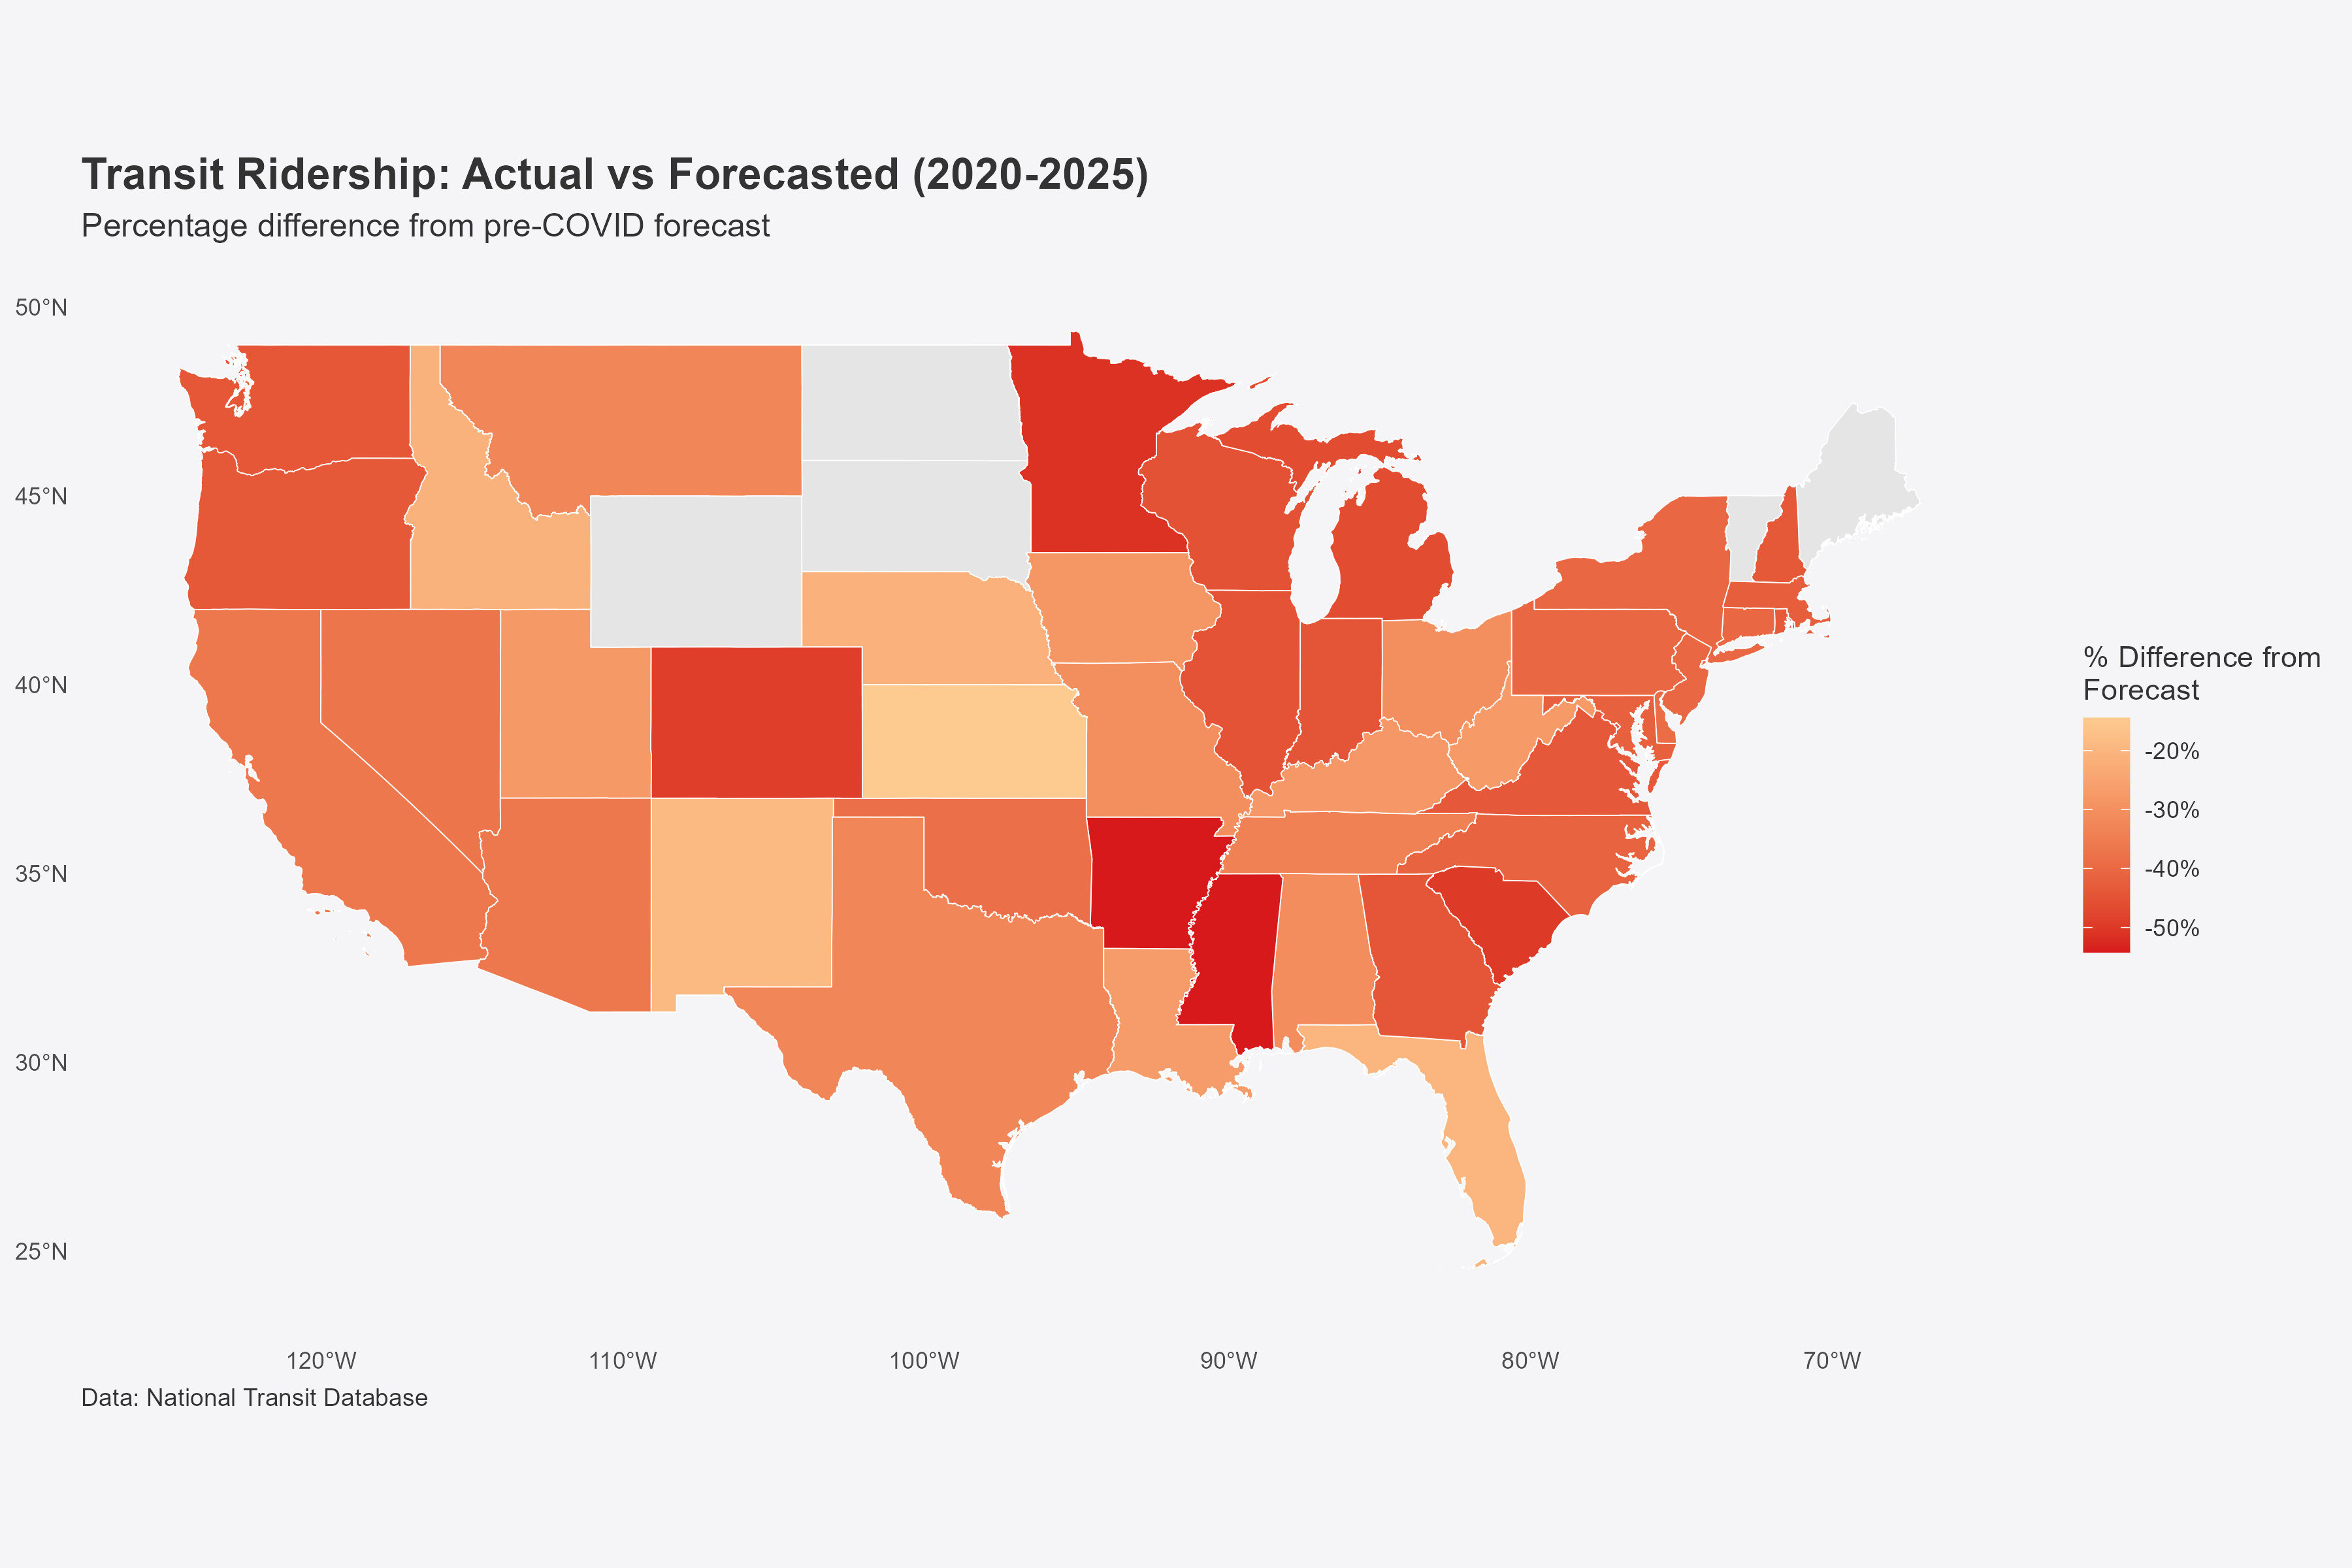
\includegraphics[width=\textwidth]{transit_ridership_map.png}
\caption{Transit Ridership: Actual vs Forecasted (2020-2025). Colors represent percentage difference from pre-COVID forecast.}
\label{fig:geographic_impact}
\end{figure}

The map reveals substantial regional disparities in pandemic impact and recovery trajectories. Midwestern and northern states such as Minnesota, Wisconsin, and Michigan experienced some of the most severe impacts, with total ridership since pandemic start is $\approx40-50\%$ below forecasted levels. In contrast, parts of the Great Plains, particularly Kansas, showed the least deviation from pre-pandemic projections ($\approx 15\%$ below forecasted levels).

Coastal regions demonstrate moderate to significant impacts, with most states experiencing ridership $20-40\%$ below pre-pandemic projections. These geographic differences likely reflect a combination of factors including varying levels of urbanization, pandemic response policies, economic structures, and transportation alternatives available in different regions.

These geographic patterns align with our jurisdiction-specific modeling results. States with larger metropolitan areas and more extensive transit networks tend to show larger negative deviations from pre-pandemic forecasts, suggesting deeper and more persistent impacts. The substantial variation in impact severity—ranging from $\approx15\%$ below forecasted levels in Kansas to nearly $50\%$ below in Minnesota and Wisconsin—mirrors the diversity we observed in optimal SARIMA model specifications across jurisdictions. This spatial heterogeneity underscores the importance of jurisdiction-specific modeling approaches rather than one-size-fits-all solutions for transit planning and recovery strategies.

%------------------------------------------------------------------------------%
\section{Discussion and Conclusions}
%------------------------------------------------------------------------------%

Our time series analysis of transit ridership provides significant insights into both typical ridership patterns and the unprecedented impact of the COVID-19 pandemic on public transportation systems across the United States. Our intervention model quantifies this shift precisely, with its highly significant COVID-19 coefficient ($\beta = -1.3321$) demonstrating an immediate $74\%$ reduction in ridership following the pandemic's onset. The model's strong predictive performance (MAPE of $7.66\%$) confirms its utility for transit planning despite unprecedented disruption. By employing multiple modeling approaches—pre-pandemic forecasting, intervention analysis, and jurisdiction-specific modeling—we have developed a comprehensive understanding of how transit ridership has evolved over time and how it continues to be affected by the pandemic's aftermath.

\subsection{Summary of Key Findings}

The primary findings from our analysis can be summarized as follows:

\begin{enumerate}
\item \textbf{Pre-pandemic patterns}: Prior to COVID-19, transit ridership across the United States demonstrated strong seasonal patterns with annual periodicity, reflecting influences of weather, academic calendars, holidays, and other cyclical factors. Our SARIMA$(2,1,0)\times(1,1,1)_{12}$ model effectively captured these patterns, although diagnostic tests suggest some remaining structure in the residuals.

\item \textbf{Immediate pandemic impact}: The onset of COVID-19 in early 2020 caused an unprecedented disruption to transit systems, with ridership plummeting to approximately 20\% of expected levels within the first two months. This decline reflected both changed travel behavior and policy decisions by transit agencies to reduce service in response to public health concerns and decreased demand.

\item \textbf{Recovery trajectory}: While ridership has steadily recovered since the initial shock, our analysis reveals that as of February 2025—nearly five years after the pandemic began—national ridership remains approximately 20\% below pre-pandemic forecasted levels. This indicates a significant and persistent impact on transit usage, even as agencies have largely restored service levels.

\item \textbf{Recovery phases}: The recovery process has followed three distinct phases: (i) initial severe impact during widespread lockdowns and service reductions, (ii) gradual recovery as restrictions eased and transit agencies restored service, and (iii) plateauing recovery with signs of stabilization at a new, lower equilibrium level. The deceleration of recovery in recent months suggests that some ridership loss may represent a permanent shift rather than a temporary anomaly.

\item \textbf{Intervention coefficient significance}: Our SARIMA(1,1,3)×(0,1,1)12 model with COVID intervention yielded a highly significant coefficient ($\beta = -1.3321, p < 0.000$), quantifying the pandemic's impact as an immediate $73.6\%$ reduction in transit ridership after accounting for existing temporal patterns, demonstrating the profound and statistically robust nature of this transportation disruption.

\item \textbf{Intervention Predictive performance}: The model's strong predictive performance (MAPE $= 7.66\%$) despite unprecedented system disruption confirms that time series methods with appropriate intervention variables can effectively capture even dramatic structural breaks in transit ridership patterns, providing a valuable framework for future disruption analysis

\item \textbf{Autoregressive dependency shift}: Our finding that $\aprrox 55\%$ of intervention models across jurisdictions showed no autoregressive dependency ($p = 0$) on previous months' ridership suggests that the pandemic fundamentally altered historical ridership relationships for many transit systems, further supporting the need for localized approaches to transit recovery.

\item \textbf{Geographic variation}: The substantial geographic variation in pandemic impact—ranging from modest $15\%$ reductions in Kansas to severe $50\%$ reductions in Minnesota and Wisconsin—reveals that regional factors significantly influence both the magnitude of disruption and recovery trajectories, highlighting the importance of jurisdiction-specific modeling rather than national averages when formulating transit policy.

\end{enumerate}

\subsection{Implications for Transit Agencies and Policy}

These findings have several important implications for transit agencies and policymakers:

\begin{enumerate}
\item \textbf{Resource allocation and service planning}: The persistent gap between current and projected pre-pandemic ridership levels requires transit agencies to reconsider resource allocation and service planning. With ridership stabilizing below previous levels, agencies may need to realign service with new demand patterns that have emerged after the pandemic.

\item \textbf{Financial sustainability}: Lower ridership directly affects fare revenue. The plateauing recovery suggests that transit agencies may need to adapt to a "new normal" of lower farebox recovery ratios, potentially requiring changes in funding models or operational efficiency. The supply-side decisions of service provision must be balanced against financial constraints in this new environment.

\item \textbf{Ridership initiatives}: Strategic initiatives to rebuild ridership may be necessary, focusing on addressing new travel patterns, remote work considerations, and potential lingering concerns about public transportation. This may include targeted service improvements in corridors where recovery has been stronger.

\item \textbf{System resilience}: The dramatic impact of COVID-19 highlights the vulnerability of transit systems to external shocks. Agencies and policymakers should consider how to build greater resilience into public transportation networks to better withstand future disruptions, including more flexible service models that can adapt quickly to changing conditions.

\item \textbf{Localized forecasting models}: The significant variation in optimal model specifications across jurisdictions underscores the need for transit agencies to develop and maintain jurisdiction-specific forecasting models rather than applying generalized patterns, particularly as recovery trajectories continue to diverge regionally following the pandemic.
\end{enumerate}

The wide variation in model specifications across jurisdictions suggests that one-size-fits-all approaches to transit planning and policy are unlikely to be effective. Recovery strategies should be tailored to local conditions, ridership patterns, and the specific service changes implemented during the pandemic.

\subsection{Limitations and Methodological Considerations}

Several limitations of our study should be acknowledged:

\begin{enumerate}
\item \textbf{Model diagnostics}: Our pre-COVID model showed some evidence of residual autocorrelation, suggesting that the model may not capture all patterns in the data. While this does not invalidate our findings, it does suggest that our forecasts should be interpreted with appropriate caution.

\item \textbf{External factors}: Our analysis focuses primarily on temporal patterns and the direct impact of COVID-19 but does not incorporate other external factors such as fuel prices, economic conditions, or specific transit service changes that may influence ridership. In particular, we do not explicitly model the extent of service reductions by transit agencies, which varied considerably across jurisdictions.

\item \textbf{Data filtering}: By limiting our analysis to jurisdictions with complete data, we may have introduced selection bias, potentially overrepresenting larger or more established transit systems with better data collection practices.

\item \textbf{Intervention specification}: Our intervention model treats the pandemic as a permanent level shift beginning in February 2020. While this captures the general pattern, it may not fully account for the complex and evolving nature of the pandemic's impact over time, including the phased reintroduction of transit service across different systems.
\end{enumerate}

\subsection{Future Research Directions}

This study suggests several promising avenues for future research:

\begin{enumerate}
\item \textbf{Multivariate analysis}: Incorporating additional variables such as employment levels, remote work trends, transit service hours, and specific policy interventions could provide a more comprehensive understanding of the factors driving changes in transit ridership.

\item \textbf{Exploring more aspects of the data}: Expanding the analysis to examine additional features in the dataset could provide additional insights about different aspects of the system. Differences in pandemic impact and recovery across transit modes could reveal important patterns in how different types of transit services respond to major disruptions and policy changes. Investigating the more directly financial features might give insights into the economics of the transit system.

\item \textbf{Changepoint and multiple seasonality methods}: Investigating additional modelling methods that incorporate a more robust changepoint analysis may help in identifying confounding factors such as policy change or changes to transit availability or service. Looking at procedures that can handle multiple seasonality may help to make the model more complete and account for more of the autocorrelation in the data.

\item \textbf{Policy effectiveness}: Evaluating how different policy responses by transit agencies influenced recovery trajectories could identify best practices for maintaining ridership during disruptions and accelerating recovery afterward.
\end{enumerate}

\subsection{Conclusion}

The COVID-19 pandemic has fundamentally altered public transit ridership patterns across the United States. While recovery has occurred, the persistent gap between current and projected pre-pandemic levels indicates a significant and potentially permanent shift in transit usage. The substantial heterogeneity in pre-pandemic patterns and post-pandemic recovery across jurisdictions underscores the complex and localized nature of transit systems and their policy responses.

The deceleration in recovery rates observed in recent months suggests that transit agencies may need to prepare for a "new normal" rather than expecting a return to pre-pandemic conditions. The geographic analysis reveals this phenomenon is not uniform—ranging from modest $10\%$ reductions in Kansas to severe $50\%$ reductions in Minnesota and Wisconsin—indicating that recovery strategies must be regionally tailored. This reality presents both challenges and opportunities for reimagining public transportation's role in a changed mobility landscape. By understanding the patterns revealed through time series analysis, transit agencies can make more informed decisions about service provision, resource allocation, and policy development as they navigate this transformation.

As public transportation continues to adapt to post-pandemic realities, time series analysis provides valuable insights for understanding both typical ridership patterns and the impact of major disruptions. The findings from this study can help transit agencies and policymakers develop data-driven strategies for rebuilding ridership, realigning service with new demand patterns, and creating more resilient transit systems for the future.
 

%------------------------------------------------------------------------------%
\appendix
%------------------------------------------------------------------------------%
\section*{Appendix}

\subsection*{A.1 Analysis details and model diagnostics}

\subsection*{Residual diagnostis for pre-COVID model}

\begin{verbatim}
	Ljung-Box test

data:  Residuals from ARIMA(2,1,0)(1,1,1)[12]  

Q* = 37.739, df = 20, p-value = 0.009529

Model df: 4.   Total lags used: 24


	Box-Ljung test

data:  residuals(best_model)  

X-squared = 37.739, df = 24, p-value = 0.03687    
\end{verbatim}

\begin{figure}[!ht]
\centering
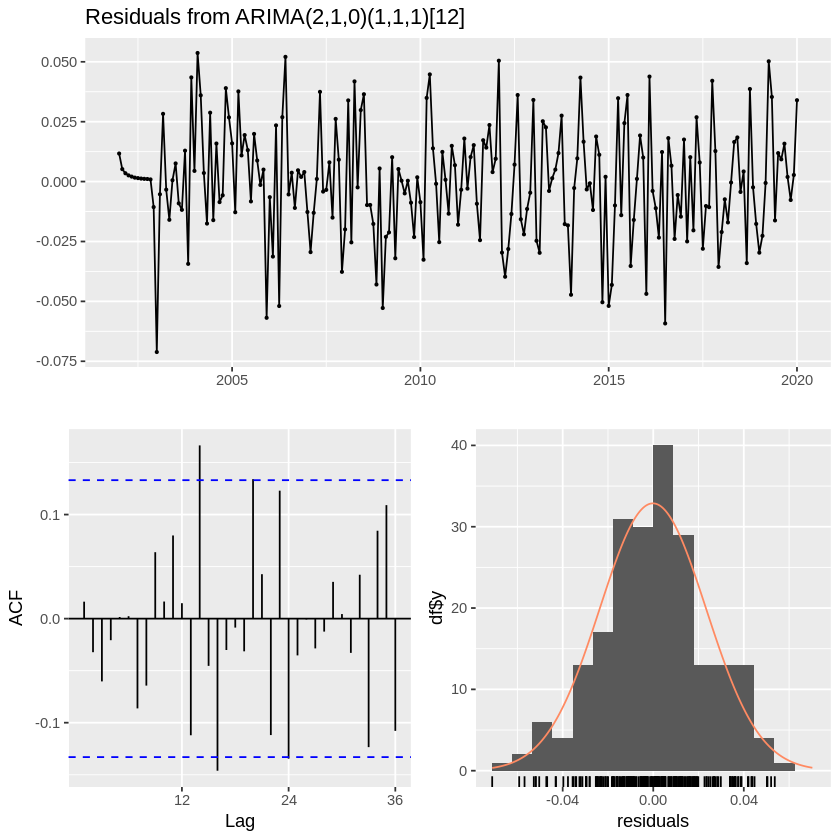
\includegraphics[width=0.485\linewidth]{residual_diag_1.png}
\caption{National transit ridership: COVID intervention forecast vs. actual values}
\label{f:pre-COVID_residual_diagnostics}
\end{figure}


\subsection*{Residual diagnostics for Intervention Model}
\begin{verbatim}
Ljung-Box test

data:  Residuals from Regression with ARIMA(1,1,3)(0,1,1)[12] errors  
Q* = 11.677, df = 19, p-value = 0.8989

Model df: 5.   Total lags used: 24


	Box-Ljung test

data:  residuals(best_model_int)  

X-squared = 11.677, df = 24, p-value = 0.9833    
\end{verbatim}



\begin{figure}[!ht]
\centering
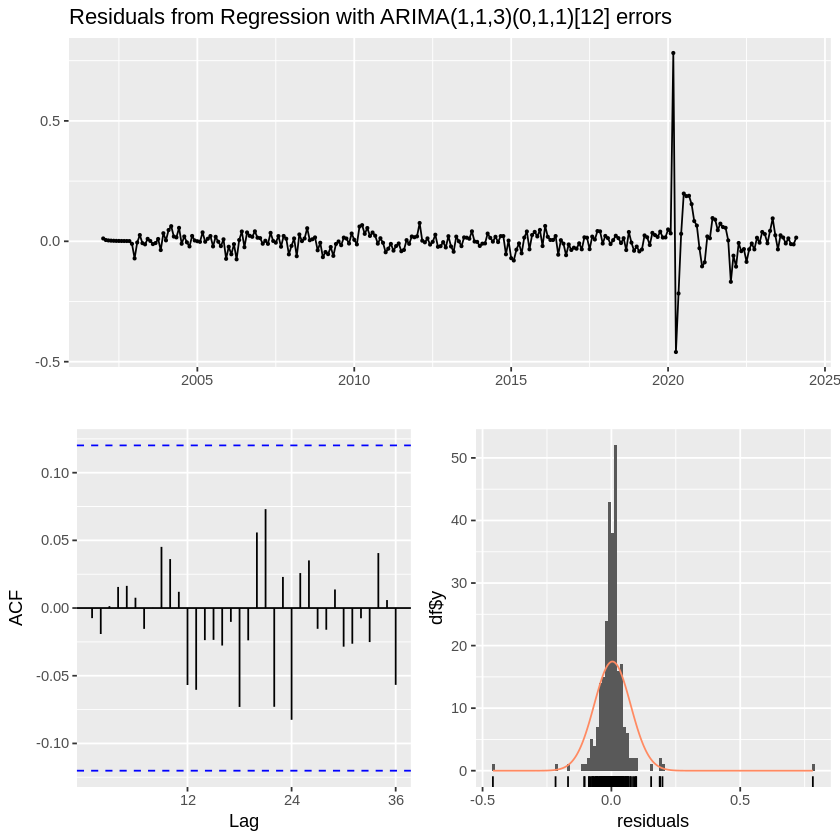
\includegraphics[width=0.485\linewidth]{residual_diag_2.png}
\caption{National transit ridership: COVID intervention forecast vs. actual values}
\label{f:intervention_residual_diagnostics}
\end{figure}


\subsection*{Replication}

The procedures for replicating the outcomes are described through the paper's Methods and Data Sections but, for the sake of brevity and accessibility, will be quickly outlined here. 

From the base data, pivot the data to create rows for each measure, sum across modes of transport for each jurisdiction, filter the jurisdictions to those that have complete and non-zero data, sum across jurisdictions to create the national sum data. 

To create the models, perform a natural logarithm transformation on the values, a lag-12 differencing to account for seasonal means, a lag-1 differencing to correct for trend components, then apply the 'Arima' function from the 'forecast' R package across the array of p, q, P, and Q values specified in the paper. Once the models are created, compare them using corrected Akaike information criterion (AICc) and use the one with the lowest value. 

\subsection*{A.2 Key R scripts for time series analysis}

{\footnotesize
\begin{verbatim}
# Load Libraries
library(tidyverse)
library(dplyr)
library(forecast)
library(ggplot2)
library(tseries)
library(lmtest)
library(knitr)
library(future)
library(furrr)

# Load data
dir.create( "/content/sta477" )
file_url <- "https://raw.githubusercontent.com/elivatsaas/sta477-final-project/refs/heads/main/Raw_Monthly_Ridership_1_2002_to_2_2025.csv"
options( download.file.method="curl", download.file.extra="-k -L" )
download.file( file_url, "/content/sta477/Raw_Monthly_Ridership_1_2002_to_1_2025.csv" )
dir( "/content/sta477" )
transit <- read.csv("/content/sta477/Raw_Monthly_Ridership_1_2002_to_1_2025.csv")[-1] %>%
  filter(!is.na(NTD.ID))

# Data cleaning
transit.tidy <- transit %>%
  pivot_longer(
    cols = 11:288,
    names_to = "months",
    values_to = "UPT")

transit.tidy <- transit.tidy %>%
  mutate(
    log_UPT = log(UPT)
  )
transit.tidy <- transit.tidy %>%
  mutate(
    # Remove the X from the month
    clean_month = gsub("^[^0-9]*([0-9]+)[^0-9]+([0-9]+)$", "\\1.\\2", months),
    month = as.numeric(sub("\\..*", "", clean_month)),
    year = as.numeric(sub(".*\\.", "", clean_month)),
    date = as.Date(paste(year, month, "01", sep = "-"))
  )

  # Get all jurisdiction for each id 
jurisdiction.modes <- transit.tidy %>%
  group_by(NTD.ID) %>%
  summarize(
    modes.list = paste(sort(unique(Mode)), collapse = ", "),
    mode.count = n_distinct(Mode),
    .groups = "drop"
  )

# Aggregate all jurisdiction data
transit.tidy.aggregated <- transit.tidy %>%
   group_by(NTD.ID, months, year, month, date)  %>%
  summarize(
    UPT.sum = sum(UPT, na.rm = TRUE),
    #Above line will return 0 if all UPT is NA, this fixes that
    UPT.sum = if_else(all(is.na(UPT)), NA_real_, UPT.sum),
    log.UPT.sum = if_else(is.na(UPT.sum), NA_real_, log(UPT.sum)),
    .groups = "drop"
  ) %>%
  left_join(jurisdiction.modes, by = "NTD.ID") %>%
  arrange(date)

# Calculate months in data
TOTAL.MONTHS <-  (2025-2002)*12+2

# Calculate missing data for each jurisdiction
aggregated.missing.data <- transit.tidy.aggregated %>%
  group_by(NTD.ID, modes.list, mode.count) %>%
  summarize(
    missing.count = sum(is.na(UPT.sum) | UPT.sum == 0, na.rm = TRUE),
    missing.percentage = ifelse(missing.count == 0, 0, missing.count / TOTAL.MONTHS),
    .groups = "drop"
  )

# Get only complete jurisdictions
complete.jurisdictions <- aggregated.missing.data %>%
  filter(missing.count == 0) %>%
  select(NTD.ID)


transit.complete <- transit.tidy.aggregated %>%
  filter(NTD.ID %in% complete.jurisdictions$NTD.ID)

# Combine all complete data into national level data
transit.all <- transit.complete %>%
  group_by(date) %>%
  summarize(total.UPT = sum(UPT.sum,na.rm = TRUE))%>%
  ungroup()%>%
  mutate(total.log.UPT = log(total.UPT))

# Total UPT plot
transit.t <- ts( transit.all$total.UPT,  start=c(2002,1), freq=12 )
plot.ts(transit.t,
        main="Total of All Jurisdiction Transit Monthly Ridership \nJan 2002 to Jan 2025",
        xlab = "Year",
        ylab = "Total UPT (millions)",
        yaxt = "n") # Suppress y-axis

# Add custom y-axis
axis(2, at = axTicks(2),
     labels = format(axTicks(2)/1000000, big.mark = ","),
     las = 1)

# log upt time series
transit.l.t <- ts( transit.all$total.log.UPT, start=c(2002,1), freq=12 )

# National Analysis
# preparing time series for analysis
transit.pre <- window(transit.t, end = c(2020, 1))

transit.l.pre <- window(transit.l.t, end = c(2020, 1))
transit.l.diff <- diff(transit.l.pre, lag = 12)

# Verify time series is not stationary already
adf.test(transit.pre)

# Plot SACF and SPACF
par(mfrow = c(2,1))
acf( transit.pre, main = "Sample ACF of Monthly Time Series", xlab = "Lag in Years", lag.max = 48)
pacf( transit.pre, main = "Sample PACF of Monthly Time Series", xlab = "Lag in Years", lag.max = 48)

# Differencing Analysis
# Apply seasonal differencing
transit.diff.alt <- diff(diff(transit.l.pre, lag = 12))

# Test for stationarity after seasonal difference
adf.test(transit.diff.alt)

# Visual Inspection for stationarity
par(mfrow = c(1, 1))
plot(transit.diff.alt, main = "Lag-1 and Lag-12 Differenced Series", ylab = "Log-Differenced Total UPT", xlab = "Year")

# Plot differenced SACF and SPACF
par(mfrow = c(2,1))
acf( transit.diff.alt, main = "Sample ACF of Lag-12 Differenced Monthly Time Series", xlab = "Lag in Years", lag.max = 48)
pacf( transit.diff.alt, main = "Sample PACF of Lag-12 Differenced Monthly Time Series", xlab = "Lag in Years", lag.max = 48)

# Apply seasonal differencing to post covid data
transit.diff.full <- diff(diff(transit.l.t, lag = 12))

# Test for stationarity after seasonal difference
adf.test(transit.diff.full)

# Visual Inspection for stationarity
par(mfrow = c(1, 1))
plot(transit.diff.full, main = "Lag-1 and Lag-12 Differenced Series COVID-19 Included",ylab = "Log-Differenced Total UPT", xlab = "Year")

# Plot SACF and SPACF for post covid
par(mfrow = c(2,1))
acf( transit.diff.full, main = "Sample ACF of Lag-12 Differenced Monthly Time Series \n COVID Included",xlab = "Lag in Years", lag.max = 48)
pacf( transit.diff.full, main = "Sample PACF of Lag-12 Differenced Monthly Time Series \n COVID Included",xlab = "Lag in Years", lag.max = 48)

# Precovid model fitting
# Model fitting - try different SARIMA models
# Model 1: SARIMA(1,1,1)(1,1,1)12
model1 <- Arima(transit.l.pre, order = c(1,1,1), seasonal = c(1,1,1))
# Model 2: SARIMA(0,1,1)(0,1,1)12
model2 <- Arima(transit.l.pre, order = c(0,1,1), seasonal = c(0,1,1))
# Model 3: SARIMA(1,1,0)(1,1,0)12
model3 <- Arima(transit.l.pre, order = c(1,1,0), seasonal = c(1,1,0))
# Model 4: SARIMA(0,1,1)(1,1,0)12
model4 <- Arima(transit.l.pre, order = c(0,1,1), seasonal = c(1,1,0))
# Model 5: SARIMA(1,1,0)(0,1,1)12
model5 <- Arima(transit.l.pre, order = c(1,1,0), seasonal = c(0,1,1))
# Model 6: SARIMA(2,1,0)(1,1,0)12
model6 <- Arima(transit.l.pre, order = c(2,1,0), seasonal = c(1,1,1))
# Model 7: SARIMA(1,1,0)(1,1,0)12
model7 <- Arima(transit.l.pre, order = c(1,1,0), seasonal = c(1,1,1))
# Model 8: SARIMA(2,1,1)(1,1,0)12
model8 <- Arima(transit.l.pre, order = c(2,1,1), seasonal = c(1,1,1))

models <- list(model1, model2, model3, model4, model5, model6, model7, model8)
aicc_values <- sapply(models, AIC, k = 2 + 2*(2+2)/(length(transit.l.pre)-2-2-1))
bic_values <- sapply(models, BIC)

model_comparison <- data.frame(
  Model = c("SARIMA(1,1,1)(1,1,1)12", "SARIMA(0,1,1)(0,1,1)12",
            "SARIMA(1,1,0)(1,1,0)12", "SARIMA(0,1,1)(1,1,0)12",
            "SARIMA(1,1,0)(0,1,1)12", "SARIMA(2,1,0)(1,1,0)12",
            "SARIMA(1,1,0)(1,1,0)12", "SARIMA(2,1,1)(1,1,0)12"),
  AICc = aicc_values,
  BIC = bic_values
)
print(model_comparison)

# Choose the best model based on AICc
best_model_index <- which.min(aicc_values)
best_model <- models[[best_model_index]]
print(best_model)

# Residual analysis for the best model
par(mfrow = c(2, 2))
checkresiduals(best_model)

# SACF and SPACF of best model
par(mfrow = c(2,1))
acf( residuals(best_model), main = "Sample ACF fo Residual Series", lag.max = 48)
pacf( residuals(best_model), main = "Sample PACF of Residual Series", lag.max = 48)

# Pre covid model forcasting
forecasts <- forecast(best_model, h = 61)
# Back-transform forecasts and prediction intervals
back_transformed_forecasts <- exp(forecasts$mean)
back_transformed_lower <- exp(forecasts$lower[,2])  # 95% interval
back_transformed_upper <- exp(forecasts$upper[,2])  # 95% interval
# Create a time series object for the back-transformed forecasts
ts_forecasts <- ts(back_transformed_forecasts, start = c(2020, 2), frequency = 12)
ts_lower <- ts(back_transformed_lower, start = c(2020, 2), frequency = 12)
ts_upper <- ts(back_transformed_upper, start = c(2020, 2), frequency = 12)

# Plot original data with forecasts
par(mfrow = c(1, 1))
plot(transit.t, xlim = c(2002, (2025+1/6)), ylim = c(min(transit.t), max(ts_upper)*1.1),
     main = "Transit Data with Forecasts",
     xlab = "Year", ylab = "Total UPT (millions)",
      yaxt = "n") # Suppress y-axis

# Add custom y-axis
axis(2, at = axTicks(2),
     labels = format(axTicks(2)/1000000, big.mark = ","),
     las = 1)
# Shade the prediction interval region
polygon(c(time(ts_lower), rev(time(ts_upper))),
        c(as.numeric(ts_lower), rev(as.numeric(ts_upper))),
        col = rgb(1, 0, 0, 0.2), border = NA)

# Add forecast and actual lines
lines(ts_forecasts, col = "blue", lwd = 2)
lines(window(transit.t, start = c(2020, 2)), col = "black", lwd = 2)
lines(ts_lower, col = "red", lty = 2)
lines(ts_upper, col = "red", lty = 2)

# Add vertical line to separate training data from forecast period
abline(v = 2020 + 1/12, lty = 3, col = "gray50")
text(2020 + 1/12, min(transit.t), "Forecast Start", pos = 4, cex = 0.8)

# Add legend
legend("topleft", legend = c("Historical Data", "Actual Future Values", "Forecast", "95% Prediction Interval"),
       col = c("black", "black", "blue", "red"),
       lty = c(1, 1, 1, 2),
       lwd = c(1, 2, 2, 1),
       fill = c(NA, NA, NA, rgb(1, 0, 0, 0.2)),
       border = c(NA, NA, NA, NA))

# Add a focused view of the forecast period
forecast_window <- window(transit.t, start = c(2019, 1))
forecast_period <- window(transit.t, start = c(2020, 2))

par(mfrow = c(1, 1))
plot(forecast_window, main = "Detailed View of Forecast Period",
     xlab = "Year", ylab = "Total UPT (millions)",
      yaxt = "n",
        ylim = c(min(c(ts_lower, forecast_period))*0.9, max(c(ts_upper, forecast_period))*1.1))
# Shade the prediction interval region
polygon(c(time(ts_lower), rev(time(ts_upper))),
        c(as.numeric(ts_lower), rev(as.numeric(ts_upper))),
        col = rgb(1, 0, 0, 0.2), border = NA)

# Add custom y-axis
axis(2, at = axTicks(2),
     labels = format(axTicks(2)/1000000, big.mark = ","),
     las = 1)

# Add forecast and actual lines
lines(ts_forecasts, col = "blue", lwd = 2)
lines(forecast_period, col = "black", lwd = 2)
lines(ts_lower, col = "red", lty = 2)
lines(ts_upper, col = "red", lty = 2)

# Add vertical line to separate training data from forecast period
abline(v = 2020, lty = 3, col = "gray50")

# Add legend
legend("topleft", legend = c("Historical Data", "Actual Future Values", "Forecast", "95% Prediction Interval"),
       col = c("black", "black", "blue", "red"),
       lty = c(1, 1, 1, 2),
       lwd = c(1, 2, 2, 1),
       fill = c(NA, NA, NA, rgb(1, 0, 0, 0.2)),
       border = c(NA, NA, NA, NA))

forecast_table <- data.frame(
  Month = rep(month.abb, length.out = length(ts_forecasts)),  # Repeat month names to match length
  Actual = round(as.numeric(window(transit.t, start = c(2020,2))), 2),
  Forecast = round(as.numeric(ts_forecasts), 2),
  Lower_95 = round(as.numeric(ts_lower), 2),
  Upper_95 = round(as.numeric(ts_upper), 2)
)


forecast_table$Estimated_Loss <- round(forecast_table$Actual - forecast_table$Forecast, 2)

forecast_table$Percentage_Loss <- ifelse(forecast_table$Forecast != 0,
                                         round((forecast_table$Estimated_Loss / forecast_table$Forecast) * 100, 1),
                                         NA)
forecast_table$Actual_Below_LowerPI <- forecast_table$Actual < forecast_table$Lower_95
forecast_table$Loss_Below_PI95 <- ifelse(forecast_table$Actual_Below_LowerPI,
                                         round(forecast_table$Lower_95 - forecast_table$Actual, 2),
                                         0)
forecast_table$Cumulative_Loss <- cumsum(forecast_table$Estimated_Loss)

forecast_table$Time_Index <- 1:nrow(forecast_table)


# Pretty print the forecast table
kable_if_available <- function(table) {
  if (requireNamespace("knitr", quietly = TRUE)) {
    return(knitr::kable(table, format = "markdown", digits = 2))
  } else {
    return(table)
  }
}
forecast_table <- forecast_table %>%
  filter(Time_Index != 1)

num_bars_plot <- nrow(forecast_table)
start_date_plot <- as.Date("2020-02-01")
date_sequence_plot <- seq.Date(from = start_date_plot, by = "month", length.out = num_bars_plot)

x_axis_labels_plot_full <- character(num_bars_plot)
for (i in 1:num_bars_plot) {
  current_date <- date_sequence_plot[i]
  month_num <- as.integer(format(current_date, "%m"))
  month_abb_str <- format(current_date, "%b")
  year_str <- format(current_date, "%Y")

  if (i == 1 && format(current_date, "%Y-%m") == "2020-02") {
    #  First label is Feb 2020
    x_axis_labels_plot_full[i] <- paste0(month_abb_str, "\n", year_str)
  } else if (month_num == 1) {
    x_axis_labels_plot_full[i] <- paste0("Jan\n", year_str)
  } else if (month_num == 7) {
    x_axis_labels_plot_full[i] <- "Jul\n "
  }
}

old_par <- par(no.readonly = TRUE)
par(mfrow = c(1, 1),
    bg = "white",
    mar = c(6.1, 4.1, 4.1, 2.1)
)

bar_centers <- barplot(forecast_table$Estimated_Loss,
                       main = "Forecast Estimated Loss (Actual - Forecast)",
                       ylab = "Estimated UPT Loss (Millions)",
                       yaxt = "n",
                       xaxt = "n",
                       col = "grey85",
                       border = "grey40",
                       ylim = c(min(0, min(forecast_table$Estimated_Loss, na.rm = TRUE)) * 1.1,
                                max(0, max(forecast_table$Estimated_Loss, na.rm = TRUE)) * 1.1),
                       col.main = "black",
                       col.lab = "black"
)

y_ticks_locations <- axTicks(2)
axis(side = 2,
     at = y_ticks_locations,
     labels = format(y_ticks_locations / 1000000, big.mark = ",", scientific = FALSE),
     las = 1,
     tick = FALSE,
     col.axis = "black",
     line = -0.5
)

label_indices <- which(x_axis_labels_plot_full != "")
tick_positions_for_x <- bar_centers[label_indices]
actual_labels_for_x <- x_axis_labels_plot_full[label_indices]

if (length(tick_positions_for_x) > 0) {
  axis(side = 1,
       at = tick_positions_for_x,
       labels = actual_labels_for_x,
       tick = TRUE,
       las = 1,
       mgp = c(3, 1.5, 0),
       col.axis = "black",
       col.ticks = "black",
       cex.axis = 0.8
  )
} else {
  warning("No labels were generated for the x-axis.")
}
abline(h = 0, lty = 2, col = "black")

# Intervention model fitting

transit.l.t.train <- window(transit.l.t, end = c(2024,2))
 # Model fitting - try different SARIMA models
n <- length(transit.l.t.train)
# Model fitting - try different SARIMA models
covid <- rep(0, n)
# Find COVID period (Feb 2020 onward - permanent effect)
t <- time(transit.l.t.train)
start_idx <- which(t >= 2020.16666)[1]  # Feb 2020
covid[start_idx:n] <- 1


# Model 1: SARIMA(1,1,1)(1,1,1)12
model1_int <- Arima(transit.l.t.train, order = c(1,1,1), seasonal = c(1,1,1), xreg=covid,
                          method="CSS-ML")
# Model 2: SARIMA(0,1,1)(0,1,1)12
model2_int <- Arima(transit.l.t.train, order = c(0,1,1), seasonal = c(0,1,1), xreg=covid,
                          method="CSS-ML")
# Model 3: SARIMA(1,1,0)(1,1,0)12
model3_int <- Arima(transit.l.t.train, order = c(1,1,0), seasonal = c(1,1,0), xreg=covid,
                          method="CSS-ML")
# Model 4: SARIMA(0,1,1)(1,1,0)12
model4_int <- Arima(transit.l.t.train, order = c(0,1,1), seasonal = c(1,1,0), xreg=covid,
                          method="CSS-ML")
# Model 5: SARIMA(1,1,0)(0,1,1)12
model5_int <- Arima(transit.l.t.train, order = c(1,1,0), seasonal = c(0,1,1), xreg=covid,
                          method="CSS-ML")
# Model 6: SARIMA(1,1,2)(0,1,1)12
model6_int <- Arima(transit.l.t.train, order = c(1,1,2), seasonal = c(0,1,1), xreg=covid,
                          method="CSS-ML")
# Model 7: SARIMA(1,1,3)(0,1,1)12
model7_int <- Arima(transit.l.t.train, order = c(1,1,3), seasonal = c(0,1,1), xreg=covid,
                          method="CSS-ML")
models_int <- list(model1_int, model2_int, model3_int, model4_int, model5_int,model6_int,model7_int)
aicc_values_int <- sapply(models_int, function(model) model$aicc)

bic_values_int <- sapply(models_int, BIC)

model_comparison_int <- data.frame(
  Model = c("SARIMA(1,1,1)(1,1,1)12", "SARIMA(0,1,1)(0,1,1)12",
            "SARIMA(1,1,0)(1,1,0)12", "SARIMA(0,1,1)(1,1,0)12",
            "SARIMA(1,1,0)(0,1,1)12","SARIMA(1,1,2)(0,1,1)12","SARIMA(1,1,3)(0,1,1)12"),
  AICc = aicc_values_int,
  BIC = bic_values_int
)
print(model_comparison_int)

# Choose the best model based on AICc
best_model_index_int <- which.min(aicc_values_int)
best_model_int <- models_int[[best_model_index_int]]
print(best_model_int)

forecast_covid <- rep(1,12)

forecasts_int <- forecast(best_model_int, h = 12, xreg = forecast_covid)

# Residual analysis for the best model
par(mfrow = c(2, 2))
checkresiduals(best_model_int)

# Back-transform forecasts and prediction intervals
back_transformed_forecasts_int <- exp(forecasts_int$mean)
back_transformed_lower_int <- exp(forecasts_int$lower[,2])  # 95% interval
back_transformed_upper_int <- exp(forecasts_int$upper[,2])  # 95% interval

# Create a time series object for the back-transformed forecasts
ts_forecasts_int <- ts(back_transformed_forecasts_int, start = c(2024, 3), frequency = 12)
ts_lower_int <- ts(back_transformed_lower_int, start = c(2024, 3), frequency = 12)
ts_upper_int <- ts(back_transformed_upper_int, start = c(2024, 3), frequency = 12)

# Plot original data with forecasts
par(mfrow = c(1, 1))
plot(transit.t, xlim = c(2002, 2025.16667), ylim = c(min(transit.t), max(ts_upper_int)*1.1),
     main = "Transit Data with Forecasts",
     xlab = "Year", ylab = "Total UPT (Millions)",          yaxt = "n") # Suppress y-axis

# Add custom y-axis
axis(2, at = axTicks(2),
     labels = format(axTicks(2)/1000000, big.mark = ","),
     las = 1)

# Shade the prediction interval region
polygon(c(time(ts_lower_int), rev(time(ts_upper_int))),
        c(as.numeric(ts_lower_int), rev(as.numeric(ts_upper_int))),
        col = rgb(1, 0, 0, 0.2), border = NA)

# Add forecast and actual lines
lines(ts_forecasts_int, col = "blue", lwd = 2)
lines(window(transit.t, start = c(2024, 3)), col = "black", lwd = 2)
lines(ts_lower_int, col = "red", lty = 2)
lines(ts_upper_int, col = "red", lty = 2)

# Add vertical line to separate training data from forecast period
abline(v = 2024 + 1/6, lty = 3, col = "gray50")  # February 2024
text(2024 + 1/6, min(ts_lower_int * 1.75), "Forecast Start →", pos = 2, cex = 0.8)



# Add legend
legend("bottomleft", legend = c("Historical Data", "Actual Future Values", "Forecast", "95% Prediction Interval"),
       col = c("black", "black", "blue", "red"),
       lty = c(1, 1, 1, 2),
       lwd = c(1, 2, 2, 1),
       fill = c(NA, NA, NA, rgb(1, 0, 0, 0.2)),
       border = c(NA, NA, NA, NA))

# Add a focused view of the forecast period
forecast_window <- window(transit.t, start = c(2022, 1))
forecast_period <- window(transit.t, start = c(2024, 3))

par(mfrow = c(1, 1))
plot(forecast_window, main = "Detailed View of Forecast Period",
     xlab = "", ylab = "Total UPT (Millions)", xaxt = "n",  # Suppress default x-axis
     ylim = c(min(c(ts_lower_int, forecast_period))*0.9, max(c(ts_upper_int, forecast_period))*1.1),          yaxt = "n") # Suppress y-axis

# Add custom y-axis
axis(2, at = axTicks(2),
     labels = format(axTicks(2)/1000000, big.mark = ","),
     las = 1)

# Create custom x-axis with month-year labels
quarter_points <- seq(2022, 2025.25, by = 0.25)  # Quarterly points
month_labels <- c()

for(t in quarter_points) {
  year <- floor(t)
  month_num <- floor(((t %% 1) * 12) + 1)
  month_name <- month.abb[month_num]
  month_labels <- c(month_labels, paste(month_name, year))
}

axis(1, at = quarter_points, labels = month_labels, las = 2, cex.axis = 0.7)

# Shade the prediction interval region
polygon(c(time(ts_lower_int), rev(time(ts_upper_int))),
        c(as.numeric(ts_lower_int), rev(as.numeric(ts_upper_int))),
        col = rgb(1, 0, 0, 0.2), border = NA)

# Add forecast and actual lines
lines(ts_forecasts_int, col = "blue", lwd = 2)
lines(forecast_period, col = "black", lwd = 2)
lines(ts_lower_int, col = "red", lty = 2)
lines(ts_upper_int, col = "red", lty = 2)
# Add vertical line to separate training data from forecast period
abline(v = 2024 + 1/6, lty = 3, col = "gray50")  # February 2024
text(2024 + 1/6, min(ts_lower_int)*0.95, "Forecast Start →", pos = 2, cex = 0.8)


# Add legend
legend("topleft", legend = c("Historical Data", "Actual Future Values", "Forecast", "95% Prediction Interval"),
       col = c("black", "black", "blue", "red"),
       lty = c(1, 1, 1, 2),
       lwd = c(1, 2, 2, 1),
       fill = c(NA, NA, NA, rgb(1, 0, 0, 0.2)),
       border = c(NA, NA, NA, NA))

# Intervention Metrics
# Define prediction period
holdout_period <- window(transit.t, start=c(2024,3), end=c(2025,2))

# Calculate accuracy metrics
# Calculate percentage errors
mape_original <- mean(abs((holdout_period - ts_forecasts_int) / holdout_period * 100))

# Convert to millions and calculate RMSE and MAE
rmse_original <- sqrt(mean((holdout_period - ts_forecasts_int)^2)) / 1e6
mae_original <- mean(abs(holdout_period - ts_forecasts_int)) / 1e6

# Display results
metrics_original <- data.frame(
  Metric = c("MAPE (%)", "RMSE (Millions)", "MAE (Millions)"),
  Value = c(round(mape_original, 2), round(rmse_original,2), round(mae_original,2))
)

print(metrics_original)

# Jurisdiction model fitting
# CAN TAKE A WHILE TO RUN WITHOUT FAST HARDWARE, REFER TO NEXT BLOCK TO DOWNLOAD FROM GITHUB

#  ARIMA model fitting function with diagnostic validation
fit_arima_both <- function(ntd_id, transit.complete, lag_check = 24, max_total_params = 5) {
  start_time <- Sys.time()
  
  # Filter data for the selected jurisdiction
  jur_data <- transit.complete %>%
    filter(NTD.ID == as.character(ntd_id)) %>%
    arrange(date)
  
  # Create time series object
  ts_data <- ts(jur_data$log.UPT.sum,
                start = c(2002, 1),
                frequency = 12)
  
  # Create the pre-COVID time series object (up to Jan 2020)
  end_pre_covid <- c(2020, 1)
  ts_pre_covid <- window(ts_data, end = end_pre_covid)
  
  # Prepare COVID dummy variable for the interruption model
  n_full <- length(ts_data)
  covid_dummy <- rep(0, n_full)
  
  # Pull out time info and set the start index for COVID
  time_full <- time(ts_data)
  start_idx_covid <- which(time_full >= 2020.16666)[1]  # Feb 2020
  if (!is.na(start_idx_covid) && start_idx_covid <= n_full) {
    covid_dummy[start_idx_covid:n_full] <- 1
  }
  
  # Function to check if residuals pass Ljung-Box test
  passes_ljung_box <- function(model, lag = lag_check) {
    if(is.null(model)) return(FALSE)
    
    # Suppress output from checkresiduals
    invisible(capture.output({
      # Use checkresiduals with plot off
      test_result <- checkresiduals(model, lag = lag, plot = FALSE)
    }))
    
    # Return TRUE if p-value > 0.05, residuals are white noise
    return(test_result$p.value > 0.05)
  }
  
  # Track models
  pre_covid_candidates <- list()
  interruption_candidates <- list()
  models_tried <- 0
  
  # Parameter limits
  max_p <- 5
  max_q <- 5
  max_P <- 2
  max_Q <- 2
  
  # First: Collect all candidate models with their AICc
  for(p in 0:max_p) {
    for(q in 0:max_q) {
      for(P in 0:max_P) {
        for(Q in 0:max_Q) {
          # Check if the total number of parameters is within the limit
          if ((p + q + P + Q) <= max_total_params) {
            models_tried <- models_tried + 1
            current_model_name <- paste0("Arima(", p, ",1,", q, ")(", P, ",1,", Q, ")[12]")
            
            # Fit Pre-COVID Model
            tryCatch({
              model_pre <- Arima(ts_pre_covid, order = c(p, 1, q), 
                                 seasonal = list(order = c(P, 1, Q), period = 12), 
                                 method = "CSS-ML")
              
              current_aicc_pre <- model_pre$aicc
              if(!is.na(current_aicc_pre)) {
                pre_covid_candidates[[length(pre_covid_candidates) + 1]] <- list(
                  model = model_pre,
                  name = current_model_name,
                  aicc = current_aicc_pre,
                  params = c(p=p, q=q, P=P, Q=Q)
                )
              }
            }, error = function(e) {})
            
            # Fit Intervention Model 
            tryCatch({
              model_inter <- Arima(ts_data, order = c(p, 1, q), 
                                   seasonal = list(order = c(P, 1, Q), period = 12), 
                                   xreg = covid_dummy, 
                                   method = "CSS-ML")
              
              current_aicc_inter <- model_inter$aicc
              if(!is.na(current_aicc_inter)) {
                interruption_candidates[[length(interruption_candidates) + 1]] <- list(
                  model = model_inter,
                  name = current_model_name,
                  aicc = current_aicc_inter,
                  params = c(p=p, q=q, P=P, Q=Q)
                )
              }
            }, error = function(e) {  })
          }
        }
      }
    }
  }
  
  # If we have no candidates, return NULL models (shouldnt happen but for robustness)
  if(length(pre_covid_candidates) == 0 || length(interruption_candidates) == 0) {
    end_time <- Sys.time()
    elapsed <- difftime(end_time, start_time, units = "secs")
    print(paste("Time Elapsed: ", elapsed, "seconds - No valid models found"))
    
    return(list(
      pre_covid = list(model = NULL, name = NULL, aicc = Inf, passes_lb = FALSE),
      interruption = list(model = NULL, name = NULL, aicc = Inf, passes_lb = FALSE),
      models_tried = models_tried,
      time_taken = elapsed
    ))
  }
  
  # Sort models by AICc (lowest first)
  pre_covid_candidates <- pre_covid_candidates[order(sapply(pre_covid_candidates, function(x) x$aicc))]
  interruption_candidates <- interruption_candidates[order(sapply(interruption_candidates, function(x) x$aicc))]
  
  # Show top 5 models by AICc
  cat("\nTop 5 intervention models by AICc for NTD.ID", ntd_id, ":\n")
  for (i in 1:min(5, length(interruption_candidates))) {
    p <- interruption_candidates[[i]]$params["p"]
    q <- interruption_candidates[[i]]$params["q"]
    P <- interruption_candidates[[i]]$params["P"]
    Q <- interruption_candidates[[i]]$params["Q"]
    cat(sprintf("ARIMA(%d,1,%d)(%d,1,%d)[12]: AICc = %.4f\n", 
                p, q, P, Q,
                interruption_candidates[[i]]$aicc))
  }
  
  
  # Start testing models in AICc order until one passes Ljung-Box
  best_pre_model <- NULL
  best_pre_name <- NULL
  best_pre_aicc <- Inf
  pre_passes_lb <- FALSE
  
  best_inter_model <- NULL
  best_inter_name <- NULL
  best_inter_aicc <- Inf
  inter_passes_lb <- FALSE
  
  # For pre-COVID models, test in AICc order until one passes
  # Store the first model as fallback
  if(length(pre_covid_candidates) > 0) {
    best_pre_model <- pre_covid_candidates[[1]]$model
    best_pre_name <- pre_covid_candidates[[1]]$name
    best_pre_aicc <- pre_covid_candidates[[1]]$aicc
    
    # Test models in order until one passes
    for(i in 1:length(pre_covid_candidates)) {
      model <- pre_covid_candidates[[i]]$model
      
      # Ljung-Box test
      lb_test_result <- passes_ljung_box(model)
      if(lb_test_result) {
        # Found a model that passes the test
        best_pre_model <- model
        best_pre_name <- pre_covid_candidates[[i]]$name
        best_pre_aicc <- pre_covid_candidates[[i]]$aicc
        pre_passes_lb <- TRUE
        break  # Early stopping once we find a passing model
      }
    }
  }
  
  # Store the first model as fallback
  if(length(interruption_candidates) > 0) {
    best_inter_model <- interruption_candidates[[1]]$model
    best_inter_name <- interruption_candidates[[1]]$name
    best_inter_aicc <- interruption_candidates[[1]]$aicc
    
    # Test all models in order until one passes
    for(i in 1:length(interruption_candidates)) {
      model <- interruption_candidates[[i]]$model
      
      # Ljung-Box test
      lb_test_result <- passes_ljung_box(model)
      if(lb_test_result) {
        # Found a model that passes the test
        best_inter_model <- model
        best_inter_name <- interruption_candidates[[i]]$name
        best_inter_aicc <- interruption_candidates[[i]]$aicc
        inter_passes_lb <- TRUE
        break  # Early stopping once we find a passing model
      }
    }
  }
  
  end_time <- Sys.time()
  elapsed <- difftime(end_time, start_time, units = "secs")
  print(paste("Time Elapsed: ", elapsed, "seconds"))
  
  # Return results with diagnostics
  return(list(
    pre_covid = list(
      model = best_pre_model, 
      name = best_pre_name, 
      aicc = best_pre_aicc,
      passes_lb = pre_passes_lb
    ),
    interruption = list(
      model = best_inter_model, 
      name = best_inter_name, 
      aicc = best_inter_aicc,
      passes_lb = inter_passes_lb
    ),
    candidates_tried_pre = length(pre_covid_candidates),
    candidates_tried_inter = length(interruption_candidates),
    models_tried = models_tried, 
    time_taken = elapsed
  ))
}

# Remove last year of data
transit.complete.train <- transit.complete %>%
  filter(date < as.Date("2024-03-01"))

# Set up parallel processing
# Use all available cores - 2
plan(multisession, workers = availableCores() - 2)

# Fit all complete jurisdictions
ids_to_process <- complete.jurisdictions$NTD.ID
start_train_time <- Sys.time()

# Parallel map
model_results <- future_map(
  ids_to_process,
  ~fit_arima_both_improved(ntd_id = .x, transit.complete = transit.complete.train),
  .progress = TRUE
)

# Set names
names(model_results) <- as.character(ids_to_process)
end_train_time <- Sys.time()

# Calculate how long training took
total_train_elapsed <- difftime(end_train_time, start_train_time, units = "secs")
print(paste("Training finished in", round(total_train_elapsed, 1), "seconds."))

file_url <- "https://github.com/elivatsaas/sta477-final-project/blob/62ef93e583b1235c167c3acf332e5999cf87b567/individual_jur_models.rds"
options( download.file.method="curl", download.file.extra="-k -L" )
download.file( file_url, "/content/sta477/individual_jur_models.rds" )
\end{verbatim}
}

%------------------------------------------------------------------------------%
% References
%------------------------------------------------------------------------------%
\spacingset{1.1}

\bibliographystyle{apalike}
\bibliography{Project-References}

\citet{Hyndman2024}

\citet{FTA2025}

%-----------------------------------------------------------------------------%
\end{document}
%-----------------------------------------------------------------------------%